% **************************************************************************************************************
% A Classic Thesis Style
% An Homage to The Elements of Typographic Style
%
% Copyright (C) 2012 Andr\'e Miede http://www.miede.de
%
% If you like the style then I would appreciate a postcard. My address 
% can be found in the file ClassicThesis.pdf. A collection of the 
% postcards I received so far is available online at 
% http://postcards.miede.de
%
% License:
% This program is free software; you can redistribute it and/or modify
% it under the terms of the GNU General Public License as published by
% the Free Software Foundation; either version 2 of the License, or
% (at your option) any later version.
%
% This program is distributed in the hope that it will be useful,
% but WITHOUT ANY WARRANTY; without even the implied warranty of
% MERCHANTABILITY or FITNESS FOR A PARTICULAR PURPOSE.  See the
% GNU General Public License for more details.
%
% You should have received a copy of the GNU General Public License
% along with this program; see the file COPYING.  If not, write to
% the Free Software Foundation, Inc., 59 Temple Place - Suite 330,
% Boston, MA 02111-1307, USA.
%
% **************************************************************************************************************
% Note:
%    * You must not use "u etc. in strings/commands that will be spaced out (use \"u or real umlauts instead)
%    * New enumeration (small caps): \begin{aenumerate} \end{aenumerate}
%    * For margin notes: \marginpar or \graffito{}
%    * Do not use bold fonts in this style, it is designed around them
%    * Use tables as in the examples
%    * See classicthesis-preamble.sty for useful commands
% **************************************************************************************************************
% To Do:
%		 * [high] Check this out: http://www.golatex.de/koma-script-warnung-in-verbindung-mit-listings-package-t2058.html
%    * [medium] mathbb in section-titles/chapter-titles => disappears somehow in headlines!!!
% **************************************************************************************************************
\documentclass[ oneside,openright,titlepage,numbers=noenddot,headinclude,%1headlines,% letterpaper a4paper
                footinclude=true,cleardoublepage=empty,abstractoff, % <--- obsolete, remove (todo)
                BCOR=5mm,paper=a4,fontsize=11pt,%11pt,a4paper,%
                ngerman,american,%
                ]{scrreprt}

%********************************************************************
% Note: Make all your adjustments in here
%*******************************************************
% ****************************************************************************************************
% classicthesis-config.tex 
% formerly known as loadpackages.sty, classicthesis-ldpkg.sty, and classicthesis-preamble.sty 
% Use it at the beginning of your ClassicThesis.tex, or as a LaTeX Preamble 
% in your ClassicThesis.{tex,lyx} with % ****************************************************************************************************
% classicthesis-config.tex 
% formerly known as loadpackages.sty, classicthesis-ldpkg.sty, and classicthesis-preamble.sty 
% Use it at the beginning of your ClassicThesis.tex, or as a LaTeX Preamble 
% in your ClassicThesis.{tex,lyx} with % ****************************************************************************************************
% classicthesis-config.tex 
% formerly known as loadpackages.sty, classicthesis-ldpkg.sty, and classicthesis-preamble.sty 
% Use it at the beginning of your ClassicThesis.tex, or as a LaTeX Preamble 
% in your ClassicThesis.{tex,lyx} with \input{classicthesis-config}
% ****************************************************************************************************  
% If you like the classicthesis, then I would appreciate a postcard. 
% My address can be found in the file ClassicThesis.pdf. A collection 
% of the postcards I received so far is available online at 
% http://postcards.miede.de
% ****************************************************************************************************

% ****************************************************************************************************
% 1. Configure classicthesis for your needs here, e.g., remove "drafting" below 
% in order to deactivate the time-stamp on the pages
% ****************************************************************************************************
\PassOptionsToPackage{eulerchapternumbers,listings,%drafting
				 pdfspacing,%floatperchapter,%linedheaders,%
				 subfig,beramono,eulermath,parts}{classicthesis}										
% ********************************************************************
% Available options for classicthesis.sty 
% (see ClassicThesis.pdf for more information):
% drafting
% parts nochapters linedheaders
% eulerchapternumbers beramono eulermath pdfspacing minionprospacing
% tocaligned dottedtoc manychapters
% listings floatperchapter subfig
% ********************************************************************

% ********************************************************************
% Triggers for this config
% ******************************************************************** 
\usepackage{ifthen}
\newboolean{enable-backrefs} % enable backrefs in the bibliography
\setboolean{enable-backrefs}{false} % true false
% ****************************************************************************************************


% ****************************************************************************************************
% 2. Personal data and user ad-hoc commands
% ****************************************************************************************************
\newcommand{\myTitle}{Interpreting natural language sentences into machine readable instructions\xspace}
%\newcommand{\mySubtitle}{An Homage to The Elements of Typographic Style\xspace}
\newcommand{\myDegree}{Master of Science in Computer Science\xspace}
\newcommand{\myName}{Martin Agfjord\xspace}
\newcommand{\mySupervisor}{Krasimir Angelov\xspace}
\newcommand{\myDepartment}{Department of Computer Science and Engineering\xspace}
\newcommand{\myUni}{University of Gothenburg\xspace}
\newcommand{\myLocation}{Gothenburg\xspace}
\newcommand{\myTime}{August 2014\xspace}
\newcommand{\myVersion}{version 1.0\xspace}

% ********************************************************************
% Setup, finetuning, and useful commands
% ********************************************************************
\newcounter{dummy} % necessary for correct hyperlinks (to index, bib, etc.)
\newlength{\abcd} % for ab..z string length calculation
\providecommand{\mLyX}{L\kern-.1667em\lower.25em\hbox{Y}\kern-.125emX\@}
\newcommand{\ie}{i.\,e.}
\newcommand{\Ie}{I.\,e.}
\newcommand{\eg}{e.\,g.}
\newcommand{\Eg}{E.\,g.} 
% ****************************************************************************************************


% ****************************************************************************************************
% 3. Loading some handy packages
% ****************************************************************************************************
% ******************************************************************** 
% Packages with options that might require adjustments
% ******************************************************************** 
%\PassOptionsToPackage{utf8}{inputenc}	% latin9 (ISO-8859-9) = latin1+"Euro sign"
\usepackage[utf8]{inputenc}	
%\PassOptionsToPackage{swedish}{babel}   % change this to your language(s)
% Spanish languages need extra options in order to work with this template
%\PassOptionsToPackage{spanish,es-lcroman}{babel}
 \usepackage[swedish]{babel}

\PassOptionsToPackage{square,numbers}{natbib}
\usepackage{natbib}
\PassOptionsToPackage{fleqn}{amsmath}		% math environments and more by the AMS 
 \usepackage{amsmath}

%\newunicodechar{00E4}{ä}
% ******************************************************************** 
% General useful packages
% ******************************************************************** 
%\PassOptionsToPackage{T1}{fontenc} % T2A for cyrillics
	\usepackage[T1]{fontenc}
\usepackage{textcomp} % fix warning with missing font shapes 
\usepackage{xspace} % to get the spacing after macros right  
\usepackage{mparhack} % get marginpar right
\usepackage{fixltx2e} % fixes some LaTeX stuff 
\PassOptionsToPackage{printonlyused,smaller}{acronym}
	\usepackage{acronym} % nice macros for handling all acronyms in the thesis
%\renewcommand*{\acsfont}[1]{\textssc{#1}} % for MinionPro
\renewcommand{\bflabel}[1]{{#1}\hfill} % fix the list of acronyms
% ****************************************************************************************************


% ****************************************************************************************************
% 4. Setup floats: tables, (sub)figures, and captions
% ****************************************************************************************************
\usepackage{tabularx} % better tables
	\setlength{\extrarowheight}{3pt} % increase table row height
\newcommand{\tableheadline}[1]{\multicolumn{1}{c}{\spacedlowsmallcaps{#1}}}
\newcommand{\myfloatalign}{\centering} % to be used with each float for alignment
\usepackage{caption}
\captionsetup{format=hang,font=small}
\usepackage{subfig}  
% ****************************************************************************************************


% ****************************************************************************************************
% 5. Setup code listings
% ****************************************************************************************************
\usepackage{listings} 
%\lstset{emph={trueIndex,root},emphstyle=\color{BlueViolet}}%\underbar} % for special keywords
\lstset{language=[LaTeX]Tex,%C++,
    keywordstyle=\color{RoyalBlue},%\bfseries,
    basicstyle=\small\ttfamily,
    %identifierstyle=\color{NavyBlue},
    commentstyle=\color{Green}\ttfamily,
    stringstyle=\rmfamily,
    numbers=none,%left,%
    numberstyle=\scriptsize,%\tiny
    stepnumber=5,
    numbersep=8pt,
    showstringspaces=false,
    breaklines=true,
    frameround=ftff,
    frame=single,
    belowcaptionskip=.75\baselineskip
    %frame=L
} 
% ****************************************************************************************************    		   


% ****************************************************************************************************
% 6. PDFLaTeX, hyperreferences and citation backreferences
% ****************************************************************************************************
% ********************************************************************
% Using PDFLaTeX
% ********************************************************************
\PassOptionsToPackage{pdftex,hyperfootnotes=false,pdfpagelabels}{hyperref}
	\usepackage{hyperref}  % backref linktocpage pagebackref
\pdfcompresslevel=9
\pdfadjustspacing=1 
\PassOptionsToPackage{pdftex}{graphicx}
	\usepackage{graphicx} 

% ********************************************************************
% Setup the style of the backrefs from the bibliography
% (translate the options to any language you use)
% ********************************************************************
\newcommand{\backrefnotcitedstring}{\relax}%(Not cited.)
\newcommand{\backrefcitedsinglestring}[1]{(Cited on page~#1.)}
\newcommand{\backrefcitedmultistring}[1]{(Cited on pages~#1.)}
\ifthenelse{\boolean{enable-backrefs}}%
{%
		\PassOptionsToPackage{hyperpageref}{backref}
		\usepackage{backref} % to be loaded after hyperref package 
		   \renewcommand{\backreftwosep}{ and~} % separate 2 pages
		   \renewcommand{\backreflastsep}{, and~} % separate last of longer list
		   \renewcommand*{\backref}[1]{}  % disable standard
		   \renewcommand*{\backrefalt}[4]{% detailed backref
		      \ifcase #1 %
		         \backrefnotcitedstring%
		      \or%
		         \backrefcitedsinglestring{#2}%
		      \else%
		         \backrefcitedmultistring{#2}%
		      \fi}%
}{\relax}    

% ********************************************************************
% Hyperreferences
% ********************************************************************
\hypersetup{%
    %draft,	% = no hyperlinking at all (useful in b/w printouts)
    colorlinks=true, linktocpage=true, pdfstartpage=3, pdfstartview=FitV,%
    % uncomment the following line if you want to have black links (e.g., for printing)
    %colorlinks=false, linktocpage=false, pdfborder={0 0 0}, pdfstartpage=3, pdfstartview=FitV,% 
    breaklinks=true, pdfpagemode=UseNone, pageanchor=true, pdfpagemode=UseOutlines,%
    plainpages=false, bookmarksnumbered, bookmarksopen=true, bookmarksopenlevel=1,%
    hypertexnames=true, pdfhighlight=/O,%nesting=true,%frenchlinks,%
    urlcolor=webbrown, linkcolor=RoyalBlue, citecolor=webgreen, %pagecolor=RoyalBlue,%
    %urlcolor=Black, linkcolor=Black, citecolor=Black, %pagecolor=Black,%
    pdftitle={\myTitle},%
    pdfauthor={\textcopyright\ \myName, \myUni, \myFaculty},%
    pdfsubject={},%
    pdfkeywords={},%
    pdfcreator={pdfLaTeX},%
    pdfproducer={LaTeX with hyperref and classicthesis}%
}   
%\hypersetup{tex4ht}


% ********************************************************************
% Setup autoreferences
% ********************************************************************
% There are some issues regarding autorefnames
% http://www.ureader.de/msg/136221647.aspx
% http://www.tex.ac.uk/cgi-bin/texfaq2html?label=latexwords
% you have to redefine the makros for the 
% language you use, e.g., american, ngerman
% (as chosen when loading babel/AtBeginDocument)
% ********************************************************************
\makeatletter
\@ifpackageloaded{babel}%
    {%
       \addto\extrasamerican{%
					\renewcommand*{\figureautorefname}{Figure}%
					\renewcommand*{\tableautorefname}{Table}%
					\renewcommand*{\partautorefname}{Part}%
					\renewcommand*{\chapterautorefname}{Chapter}%
					\renewcommand*{\sectionautorefname}{Section}%
					\renewcommand*{\subsectionautorefname}{Section}%
					\renewcommand*{\subsubsectionautorefname}{Section}% 	
				}%
       \addto\extrasngerman{% 
					\renewcommand*{\paragraphautorefname}{Absatz}%
					\renewcommand*{\subparagraphautorefname}{Unterabsatz}%
					\renewcommand*{\footnoteautorefname}{Fu\"snote}%
					\renewcommand*{\FancyVerbLineautorefname}{Zeile}%
					\renewcommand*{\theoremautorefname}{Theorem}%
					\renewcommand*{\appendixautorefname}{Anhang}%
					\renewcommand*{\equationautorefname}{Gleichung}%        
					\renewcommand*{\itemautorefname}{Punkt}%
				}%	
			% Fix to getting autorefs for subfigures right (thanks to Belinda Vogt for changing the definition)
			\providecommand{\subfigureautorefname}{\figureautorefname}%  			
    }{\relax}
\makeatother


% ****************************************************************************************************
% 7. Last calls before the bar closes
% ****************************************************************************************************
% ********************************************************************
% Development Stuff
% ********************************************************************
\listfiles
%\PassOptionsToPackage{l2tabu,orthodox,abort}{nag}
%	\usepackage{nag}
%\PassOptionsToPackage{warning, all}{onlyamsmath}
%	\usepackage{onlyamsmath}

% ********************************************************************
% Last, but not least...
% ********************************************************************
\usepackage{classicthesis} 
% ****************************************************************************************************


% ****************************************************************************************************
% 8. Further adjustments (experimental)
% ****************************************************************************************************
% ********************************************************************
% Changing the text area
% ********************************************************************
%\linespread{1.05} % a bit more for Palatino
%\areaset[current]{312pt}{761pt} % 686 (factor 2.2) + 33 head + 42 head \the\footskip
%\setlength{\marginparwidth}{7em}%
%\setlength{\marginparsep}{2em}%

% ********************************************************************
% Using different fonts
% ********************************************************************
%\usepackage[oldstylenums]{kpfonts} % oldstyle notextcomp
%\usepackage[osf]{libertine}
%\usepackage{hfoldsty} % Computer Modern with osf
%\usepackage[light,condensed,math]{iwona}
%\renewcommand{\sfdefault}{iwona}
%\usepackage{lmodern} % <-- no osf support :-(
%\usepackage[urw-garamond]{mathdesign} <-- no osf support :-(
% ****************************************************************************************************

% *********************************************************************
% Syntax highlighting
% *********************************************************************
% \usepackage{fontspec}
\usepackage{minted}

%
% Fix to support extended characters in minted with combination of pdfTeX
% http://tex.stackexchange.com/questions/19781/using-package-minted-with-non-english-characters
%

\makeatletter
\newcommand{\minted@write@detok}[1]{%
  \immediate\write\FV@OutFile{\detokenize{#1}}}%

% Blank page
\newcommand*{\blankpage}{%
  \begingroup
    \setlength{\topskip}{0pt}%
    \setlength{\parskip}{0pt}%
    \vspace*{\fill}%
    \centering
    \nointerlineskip % suppresses partial \baselineskip above text
    This page is intentionally left (almost) blank.\par
    \thispagestyle{empty}
    \setcounter{page}{}
    \vspace{\fill}%
  \endgroup
  % \showlists
}

\newcommand{\minted@FVB@VerbatimOut}[1]{%
  \@bsphack
  \begingroup
    \FV@UseKeyValues
    \FV@DefineWhiteSpace
    \def\FV@Space{\space}%
    \FV@DefineTabOut
    %\def\FV@ProcessLine{\immediate\write\FV@OutFile}% %Old, non-Unicode version
    \let\FV@ProcessLine\minted@write@detok %Patch for Unicode
    \immediate\openout\FV@OutFile #1\relax
    \let\FV@FontScanPrep\relax
%% DG/SR modification begin - May. 18, 1998 (to avoid problems with ligatures)
    \let\@noligs\relax
%% DG/SR modification end
    \FV@Scan}
    \let\FVB@VerbatimOut\minted@FVB@VerbatimOut

\renewcommand\minted@savecode[1]{
  \immediate\openout\minted@code\jobname.pyg
  \immediate\write\minted@code{\expandafter\detokenize\expandafter{#1}}%
  \immediate\closeout\minted@code}
\makeatother

\usepackage{tcolorbox}
\tcbuselibrary{skins}
\usetikzlibrary{shadings}

\usepackage{etoolbox}

% Code
\BeforeBeginEnvironment{code}{\begin{tcolorbox}[enhanced,
width=\linewidth,
enlarge top by=3pt,enlarge bottom by=3pt,
enlarge left by=3pt,enlarge right by=3pt,
frame hidden,boxrule=0pt,top=1mm,bottom=1mm,
colframe=green!30!black, colbacktitle=green!50!yellow,
coltitle=black, colback=bg,
borderline={.1pt}{-0.5pt}{gray, dashed, sharp corners}]}%
\AfterEndEnvironment{code}{\end{tcolorbox}}

% Terminal
\BeforeBeginEnvironment{terminal}{\begin{tcolorbox}[enhanced,
width=\linewidth,
enlarge top by=3pt,enlarge bottom by=3pt,
enlarge left by=3pt,enlarge right by=3pt,
frame hidden,boxrule=0pt,top=1mm,bottom=1mm,
colframe=green!30!black, colbacktitle=green!50!yellow,
coltitle=black, colback=bg,
borderline={.1pt}{-0.5pt}{gray, dashed, sharp corners}]}%
\AfterEndEnvironment{terminal}{\end{tcolorbox}}

% Java
\BeforeBeginEnvironment{java-code}{\begin{tcolorbox}[enhanced,
width=\linewidth,
enlarge top by=3pt,enlarge bottom by=3pt,
enlarge left by=3pt,enlarge right by=3pt,
frame hidden,boxrule=0pt,top=1mm,bottom=1mm,
colframe=green!30!black, colbacktitle=green!50!yellow,
coltitle=black, colback=bg,
borderline={.1pt}{-0.5pt}{gray, dashed, sharp corners}]}%
\AfterEndEnvironment{java-code}{\end{tcolorbox}}

% Js
\BeforeBeginEnvironment{js-code}{\begin{tcolorbox}[enhanced,
width=\linewidth,
enlarge top by=3pt,enlarge bottom by=3pt,
enlarge left by=3pt,enlarge right by=3pt,
frame hidden,boxrule=0pt,top=1mm,bottom=1mm,
colframe=green!30!black, colbacktitle=green!50!yellow,
coltitle=black, colback=bg,
borderline={.1pt}{-0.5pt}{gray, dashed, sharp corners}]}%
\AfterEndEnvironment{js-code}{\end{tcolorbox}}

% Json
\BeforeBeginEnvironment{json-normal}{\begin{tcolorbox}[enhanced,
width=\linewidth,
enlarge top by=3pt,enlarge bottom by=3pt,
enlarge left by=3pt,enlarge right by=3pt,
frame hidden,boxrule=0pt,top=1mm,bottom=1mm,
colframe=green!30!black, colbacktitle=green!50!yellow,
coltitle=black, colback=bg,
borderline={.1pt}{-0.5pt}{gray, dashed, sharp corners}]}%
\AfterEndEnvironment{json-normal}{\end{tcolorbox}}

% Json
\BeforeBeginEnvironment{json-small}{\begin{tcolorbox}[enhanced,
width=\linewidth,
enlarge top by=3pt,enlarge bottom by=3pt,
enlarge left by=3pt,enlarge right by=3pt,
frame hidden,boxrule=0pt,top=1mm,bottom=1mm,
colframe=green!30!black, colbacktitle=green!50!yellow,
coltitle=black, colback=bg,
borderline={.1pt}{-0.5pt}{gray, dashed, sharp corners}]}%
\AfterEndEnvironment{json-small}{\end{tcolorbox}}


% Plaintext
\BeforeBeginEnvironment{plaintext}{\begin{tcolorbox}[enhanced,
frame hidden,boxrule=0pt,top=1mm,bottom=0.5mm]}%
\AfterEndEnvironment{plaintext}{\end{tcolorbox}}%

\definecolor{bg}{HTML}{F2F2F2}
\newminted[code]{text}{mathescape=true,linenos=true,numbersep=5pt,fontsize=\footnotesize,framesep=10pt}
\newminted[java-code]{csharp}{linenos=true,numbersep=5pt,fontsize=\footnotesize,framesep=10pt}
\newminted[js-code]{js}{linenos=true,numbersep=5pt,fontsize=\footnotesize,framesep=10pt}
\newminted[json-normal]{js}{linenos=true,numbersep=5pt,fontsize=\footnotesize,framesep=10pt}
\newminted[json-small]{js}{linenos=true,numbersep=5pt,fontsize=\scriptsize,framesep=10pt}
\newminted[terminal]{text}{linenos=false,numbersep=5pt,fontsize=\footnotesize,framesep=10pt}
\newminted[plaintext]{text}{linenos=false,numbersep=5pt,fontsize=\footnotesize,framesep=10pt}
\newminted[bashcode2]{bash}{linenos=true, texcl=true}
\usepackage{scrhack} % fix warnings when using KOMA with listings package         
%\setsansfont{Calibri}
%\setmonofont{Consolas}
%\renewcommand{\familydefault}{\sfdefault}

\usepackage{etoolbox}

% Margin
\usepackage[left=1.5in,right=1.5in,top=1.5in,bottom=1.5in]{geometry}
\usepackage[framemethod=default]{mdframed}

%Exact positioning
\usepackage{float}

%Hyper-links
\usepackage{hyperref}

%Todo color
\usepackage{xcolor}
\newcommand\todo[1]{\textcolor{red}{#1}}

% Centering of graphics
\usepackage[export]{adjustbox}% http://ctan.org/pkg/adjustbox

%Hidden sections
\newcommand{\hiddensubsection}[1]{
    \stepcounter{subsection}
    \subsection*{\arabic{chapter}.\arabic{section}.\arabic{subsection}\hspace{1em}{#1}}
}

\newcommand{\hiddensubsubsection}[1]{
    \stepcounter{subsubsection}
    \subsubsection*{\arabic{chapter}.\arabic{section}.\arabic{subsection}\hspace{1em}{#1}}
}

\newcommand{\hiddensubsubsubsection}[1]{
    \stepcounter{subsubsubsection}
    \subsubsubsection*{\arabic{chapter}.\arabic{section}.\arabic{subsection}\hspace{1em}{#1}}
}

% Include pdfs
\usepackage{pdfpages}
% ****************************************************************************************************  
% If you like the classicthesis, then I would appreciate a postcard. 
% My address can be found in the file ClassicThesis.pdf. A collection 
% of the postcards I received so far is available online at 
% http://postcards.miede.de
% ****************************************************************************************************

% ****************************************************************************************************
% 1. Configure classicthesis for your needs here, e.g., remove "drafting" below 
% in order to deactivate the time-stamp on the pages
% ****************************************************************************************************
\PassOptionsToPackage{eulerchapternumbers,listings,%drafting
				 pdfspacing,%floatperchapter,%linedheaders,%
				 subfig,beramono,eulermath,parts}{classicthesis}										
% ********************************************************************
% Available options for classicthesis.sty 
% (see ClassicThesis.pdf for more information):
% drafting
% parts nochapters linedheaders
% eulerchapternumbers beramono eulermath pdfspacing minionprospacing
% tocaligned dottedtoc manychapters
% listings floatperchapter subfig
% ********************************************************************

% ********************************************************************
% Triggers for this config
% ******************************************************************** 
\usepackage{ifthen}
\newboolean{enable-backrefs} % enable backrefs in the bibliography
\setboolean{enable-backrefs}{false} % true false
% ****************************************************************************************************


% ****************************************************************************************************
% 2. Personal data and user ad-hoc commands
% ****************************************************************************************************
\newcommand{\myTitle}{Interpreting natural language sentences into machine readable instructions\xspace}
%\newcommand{\mySubtitle}{An Homage to The Elements of Typographic Style\xspace}
\newcommand{\myDegree}{Master of Science in Computer Science\xspace}
\newcommand{\myName}{Martin Agfjord\xspace}
\newcommand{\mySupervisor}{Krasimir Angelov\xspace}
\newcommand{\myDepartment}{Department of Computer Science and Engineering\xspace}
\newcommand{\myUni}{University of Gothenburg\xspace}
\newcommand{\myLocation}{Gothenburg\xspace}
\newcommand{\myTime}{August 2014\xspace}
\newcommand{\myVersion}{version 1.0\xspace}

% ********************************************************************
% Setup, finetuning, and useful commands
% ********************************************************************
\newcounter{dummy} % necessary for correct hyperlinks (to index, bib, etc.)
\newlength{\abcd} % for ab..z string length calculation
\providecommand{\mLyX}{L\kern-.1667em\lower.25em\hbox{Y}\kern-.125emX\@}
\newcommand{\ie}{i.\,e.}
\newcommand{\Ie}{I.\,e.}
\newcommand{\eg}{e.\,g.}
\newcommand{\Eg}{E.\,g.} 
% ****************************************************************************************************


% ****************************************************************************************************
% 3. Loading some handy packages
% ****************************************************************************************************
% ******************************************************************** 
% Packages with options that might require adjustments
% ******************************************************************** 
%\PassOptionsToPackage{utf8}{inputenc}	% latin9 (ISO-8859-9) = latin1+"Euro sign"
\usepackage[utf8]{inputenc}	
%\PassOptionsToPackage{swedish}{babel}   % change this to your language(s)
% Spanish languages need extra options in order to work with this template
%\PassOptionsToPackage{spanish,es-lcroman}{babel}
 \usepackage[swedish]{babel}

\PassOptionsToPackage{square,numbers}{natbib}
\usepackage{natbib}
\PassOptionsToPackage{fleqn}{amsmath}		% math environments and more by the AMS 
 \usepackage{amsmath}

%\newunicodechar{00E4}{ä}
% ******************************************************************** 
% General useful packages
% ******************************************************************** 
%\PassOptionsToPackage{T1}{fontenc} % T2A for cyrillics
	\usepackage[T1]{fontenc}
\usepackage{textcomp} % fix warning with missing font shapes 
\usepackage{xspace} % to get the spacing after macros right  
\usepackage{mparhack} % get marginpar right
\usepackage{fixltx2e} % fixes some LaTeX stuff 
\PassOptionsToPackage{printonlyused,smaller}{acronym}
	\usepackage{acronym} % nice macros for handling all acronyms in the thesis
%\renewcommand*{\acsfont}[1]{\textssc{#1}} % for MinionPro
\renewcommand{\bflabel}[1]{{#1}\hfill} % fix the list of acronyms
% ****************************************************************************************************


% ****************************************************************************************************
% 4. Setup floats: tables, (sub)figures, and captions
% ****************************************************************************************************
\usepackage{tabularx} % better tables
	\setlength{\extrarowheight}{3pt} % increase table row height
\newcommand{\tableheadline}[1]{\multicolumn{1}{c}{\spacedlowsmallcaps{#1}}}
\newcommand{\myfloatalign}{\centering} % to be used with each float for alignment
\usepackage{caption}
\captionsetup{format=hang,font=small}
\usepackage{subfig}  
% ****************************************************************************************************


% ****************************************************************************************************
% 5. Setup code listings
% ****************************************************************************************************
\usepackage{listings} 
%\lstset{emph={trueIndex,root},emphstyle=\color{BlueViolet}}%\underbar} % for special keywords
\lstset{language=[LaTeX]Tex,%C++,
    keywordstyle=\color{RoyalBlue},%\bfseries,
    basicstyle=\small\ttfamily,
    %identifierstyle=\color{NavyBlue},
    commentstyle=\color{Green}\ttfamily,
    stringstyle=\rmfamily,
    numbers=none,%left,%
    numberstyle=\scriptsize,%\tiny
    stepnumber=5,
    numbersep=8pt,
    showstringspaces=false,
    breaklines=true,
    frameround=ftff,
    frame=single,
    belowcaptionskip=.75\baselineskip
    %frame=L
} 
% ****************************************************************************************************    		   


% ****************************************************************************************************
% 6. PDFLaTeX, hyperreferences and citation backreferences
% ****************************************************************************************************
% ********************************************************************
% Using PDFLaTeX
% ********************************************************************
\PassOptionsToPackage{pdftex,hyperfootnotes=false,pdfpagelabels}{hyperref}
	\usepackage{hyperref}  % backref linktocpage pagebackref
\pdfcompresslevel=9
\pdfadjustspacing=1 
\PassOptionsToPackage{pdftex}{graphicx}
	\usepackage{graphicx} 

% ********************************************************************
% Setup the style of the backrefs from the bibliography
% (translate the options to any language you use)
% ********************************************************************
\newcommand{\backrefnotcitedstring}{\relax}%(Not cited.)
\newcommand{\backrefcitedsinglestring}[1]{(Cited on page~#1.)}
\newcommand{\backrefcitedmultistring}[1]{(Cited on pages~#1.)}
\ifthenelse{\boolean{enable-backrefs}}%
{%
		\PassOptionsToPackage{hyperpageref}{backref}
		\usepackage{backref} % to be loaded after hyperref package 
		   \renewcommand{\backreftwosep}{ and~} % separate 2 pages
		   \renewcommand{\backreflastsep}{, and~} % separate last of longer list
		   \renewcommand*{\backref}[1]{}  % disable standard
		   \renewcommand*{\backrefalt}[4]{% detailed backref
		      \ifcase #1 %
		         \backrefnotcitedstring%
		      \or%
		         \backrefcitedsinglestring{#2}%
		      \else%
		         \backrefcitedmultistring{#2}%
		      \fi}%
}{\relax}    

% ********************************************************************
% Hyperreferences
% ********************************************************************
\hypersetup{%
    %draft,	% = no hyperlinking at all (useful in b/w printouts)
    colorlinks=true, linktocpage=true, pdfstartpage=3, pdfstartview=FitV,%
    % uncomment the following line if you want to have black links (e.g., for printing)
    %colorlinks=false, linktocpage=false, pdfborder={0 0 0}, pdfstartpage=3, pdfstartview=FitV,% 
    breaklinks=true, pdfpagemode=UseNone, pageanchor=true, pdfpagemode=UseOutlines,%
    plainpages=false, bookmarksnumbered, bookmarksopen=true, bookmarksopenlevel=1,%
    hypertexnames=true, pdfhighlight=/O,%nesting=true,%frenchlinks,%
    urlcolor=webbrown, linkcolor=RoyalBlue, citecolor=webgreen, %pagecolor=RoyalBlue,%
    %urlcolor=Black, linkcolor=Black, citecolor=Black, %pagecolor=Black,%
    pdftitle={\myTitle},%
    pdfauthor={\textcopyright\ \myName, \myUni, \myFaculty},%
    pdfsubject={},%
    pdfkeywords={},%
    pdfcreator={pdfLaTeX},%
    pdfproducer={LaTeX with hyperref and classicthesis}%
}   
%\hypersetup{tex4ht}


% ********************************************************************
% Setup autoreferences
% ********************************************************************
% There are some issues regarding autorefnames
% http://www.ureader.de/msg/136221647.aspx
% http://www.tex.ac.uk/cgi-bin/texfaq2html?label=latexwords
% you have to redefine the makros for the 
% language you use, e.g., american, ngerman
% (as chosen when loading babel/AtBeginDocument)
% ********************************************************************
\makeatletter
\@ifpackageloaded{babel}%
    {%
       \addto\extrasamerican{%
					\renewcommand*{\figureautorefname}{Figure}%
					\renewcommand*{\tableautorefname}{Table}%
					\renewcommand*{\partautorefname}{Part}%
					\renewcommand*{\chapterautorefname}{Chapter}%
					\renewcommand*{\sectionautorefname}{Section}%
					\renewcommand*{\subsectionautorefname}{Section}%
					\renewcommand*{\subsubsectionautorefname}{Section}% 	
				}%
       \addto\extrasngerman{% 
					\renewcommand*{\paragraphautorefname}{Absatz}%
					\renewcommand*{\subparagraphautorefname}{Unterabsatz}%
					\renewcommand*{\footnoteautorefname}{Fu\"snote}%
					\renewcommand*{\FancyVerbLineautorefname}{Zeile}%
					\renewcommand*{\theoremautorefname}{Theorem}%
					\renewcommand*{\appendixautorefname}{Anhang}%
					\renewcommand*{\equationautorefname}{Gleichung}%        
					\renewcommand*{\itemautorefname}{Punkt}%
				}%	
			% Fix to getting autorefs for subfigures right (thanks to Belinda Vogt for changing the definition)
			\providecommand{\subfigureautorefname}{\figureautorefname}%  			
    }{\relax}
\makeatother


% ****************************************************************************************************
% 7. Last calls before the bar closes
% ****************************************************************************************************
% ********************************************************************
% Development Stuff
% ********************************************************************
\listfiles
%\PassOptionsToPackage{l2tabu,orthodox,abort}{nag}
%	\usepackage{nag}
%\PassOptionsToPackage{warning, all}{onlyamsmath}
%	\usepackage{onlyamsmath}

% ********************************************************************
% Last, but not least...
% ********************************************************************
\usepackage{classicthesis} 
% ****************************************************************************************************


% ****************************************************************************************************
% 8. Further adjustments (experimental)
% ****************************************************************************************************
% ********************************************************************
% Changing the text area
% ********************************************************************
%\linespread{1.05} % a bit more for Palatino
%\areaset[current]{312pt}{761pt} % 686 (factor 2.2) + 33 head + 42 head \the\footskip
%\setlength{\marginparwidth}{7em}%
%\setlength{\marginparsep}{2em}%

% ********************************************************************
% Using different fonts
% ********************************************************************
%\usepackage[oldstylenums]{kpfonts} % oldstyle notextcomp
%\usepackage[osf]{libertine}
%\usepackage{hfoldsty} % Computer Modern with osf
%\usepackage[light,condensed,math]{iwona}
%\renewcommand{\sfdefault}{iwona}
%\usepackage{lmodern} % <-- no osf support :-(
%\usepackage[urw-garamond]{mathdesign} <-- no osf support :-(
% ****************************************************************************************************

% *********************************************************************
% Syntax highlighting
% *********************************************************************
% \usepackage{fontspec}
\usepackage{minted}

%
% Fix to support extended characters in minted with combination of pdfTeX
% http://tex.stackexchange.com/questions/19781/using-package-minted-with-non-english-characters
%

\makeatletter
\newcommand{\minted@write@detok}[1]{%
  \immediate\write\FV@OutFile{\detokenize{#1}}}%

% Blank page
\newcommand*{\blankpage}{%
  \begingroup
    \setlength{\topskip}{0pt}%
    \setlength{\parskip}{0pt}%
    \vspace*{\fill}%
    \centering
    \nointerlineskip % suppresses partial \baselineskip above text
    This page is intentionally left (almost) blank.\par
    \thispagestyle{empty}
    \setcounter{page}{}
    \vspace{\fill}%
  \endgroup
  % \showlists
}

\newcommand{\minted@FVB@VerbatimOut}[1]{%
  \@bsphack
  \begingroup
    \FV@UseKeyValues
    \FV@DefineWhiteSpace
    \def\FV@Space{\space}%
    \FV@DefineTabOut
    %\def\FV@ProcessLine{\immediate\write\FV@OutFile}% %Old, non-Unicode version
    \let\FV@ProcessLine\minted@write@detok %Patch for Unicode
    \immediate\openout\FV@OutFile #1\relax
    \let\FV@FontScanPrep\relax
%% DG/SR modification begin - May. 18, 1998 (to avoid problems with ligatures)
    \let\@noligs\relax
%% DG/SR modification end
    \FV@Scan}
    \let\FVB@VerbatimOut\minted@FVB@VerbatimOut

\renewcommand\minted@savecode[1]{
  \immediate\openout\minted@code\jobname.pyg
  \immediate\write\minted@code{\expandafter\detokenize\expandafter{#1}}%
  \immediate\closeout\minted@code}
\makeatother

\usepackage{tcolorbox}
\tcbuselibrary{skins}
\usetikzlibrary{shadings}

\usepackage{etoolbox}

% Code
\BeforeBeginEnvironment{code}{\begin{tcolorbox}[enhanced,
width=\linewidth,
enlarge top by=3pt,enlarge bottom by=3pt,
enlarge left by=3pt,enlarge right by=3pt,
frame hidden,boxrule=0pt,top=1mm,bottom=1mm,
colframe=green!30!black, colbacktitle=green!50!yellow,
coltitle=black, colback=bg,
borderline={.1pt}{-0.5pt}{gray, dashed, sharp corners}]}%
\AfterEndEnvironment{code}{\end{tcolorbox}}

% Terminal
\BeforeBeginEnvironment{terminal}{\begin{tcolorbox}[enhanced,
width=\linewidth,
enlarge top by=3pt,enlarge bottom by=3pt,
enlarge left by=3pt,enlarge right by=3pt,
frame hidden,boxrule=0pt,top=1mm,bottom=1mm,
colframe=green!30!black, colbacktitle=green!50!yellow,
coltitle=black, colback=bg,
borderline={.1pt}{-0.5pt}{gray, dashed, sharp corners}]}%
\AfterEndEnvironment{terminal}{\end{tcolorbox}}

% Java
\BeforeBeginEnvironment{java-code}{\begin{tcolorbox}[enhanced,
width=\linewidth,
enlarge top by=3pt,enlarge bottom by=3pt,
enlarge left by=3pt,enlarge right by=3pt,
frame hidden,boxrule=0pt,top=1mm,bottom=1mm,
colframe=green!30!black, colbacktitle=green!50!yellow,
coltitle=black, colback=bg,
borderline={.1pt}{-0.5pt}{gray, dashed, sharp corners}]}%
\AfterEndEnvironment{java-code}{\end{tcolorbox}}

% Js
\BeforeBeginEnvironment{js-code}{\begin{tcolorbox}[enhanced,
width=\linewidth,
enlarge top by=3pt,enlarge bottom by=3pt,
enlarge left by=3pt,enlarge right by=3pt,
frame hidden,boxrule=0pt,top=1mm,bottom=1mm,
colframe=green!30!black, colbacktitle=green!50!yellow,
coltitle=black, colback=bg,
borderline={.1pt}{-0.5pt}{gray, dashed, sharp corners}]}%
\AfterEndEnvironment{js-code}{\end{tcolorbox}}

% Json
\BeforeBeginEnvironment{json-normal}{\begin{tcolorbox}[enhanced,
width=\linewidth,
enlarge top by=3pt,enlarge bottom by=3pt,
enlarge left by=3pt,enlarge right by=3pt,
frame hidden,boxrule=0pt,top=1mm,bottom=1mm,
colframe=green!30!black, colbacktitle=green!50!yellow,
coltitle=black, colback=bg,
borderline={.1pt}{-0.5pt}{gray, dashed, sharp corners}]}%
\AfterEndEnvironment{json-normal}{\end{tcolorbox}}

% Json
\BeforeBeginEnvironment{json-small}{\begin{tcolorbox}[enhanced,
width=\linewidth,
enlarge top by=3pt,enlarge bottom by=3pt,
enlarge left by=3pt,enlarge right by=3pt,
frame hidden,boxrule=0pt,top=1mm,bottom=1mm,
colframe=green!30!black, colbacktitle=green!50!yellow,
coltitle=black, colback=bg,
borderline={.1pt}{-0.5pt}{gray, dashed, sharp corners}]}%
\AfterEndEnvironment{json-small}{\end{tcolorbox}}


% Plaintext
\BeforeBeginEnvironment{plaintext}{\begin{tcolorbox}[enhanced,
frame hidden,boxrule=0pt,top=1mm,bottom=0.5mm]}%
\AfterEndEnvironment{plaintext}{\end{tcolorbox}}%

\definecolor{bg}{HTML}{F2F2F2}
\newminted[code]{text}{mathescape=true,linenos=true,numbersep=5pt,fontsize=\footnotesize,framesep=10pt}
\newminted[java-code]{csharp}{linenos=true,numbersep=5pt,fontsize=\footnotesize,framesep=10pt}
\newminted[js-code]{js}{linenos=true,numbersep=5pt,fontsize=\footnotesize,framesep=10pt}
\newminted[json-normal]{js}{linenos=true,numbersep=5pt,fontsize=\footnotesize,framesep=10pt}
\newminted[json-small]{js}{linenos=true,numbersep=5pt,fontsize=\scriptsize,framesep=10pt}
\newminted[terminal]{text}{linenos=false,numbersep=5pt,fontsize=\footnotesize,framesep=10pt}
\newminted[plaintext]{text}{linenos=false,numbersep=5pt,fontsize=\footnotesize,framesep=10pt}
\newminted[bashcode2]{bash}{linenos=true, texcl=true}
\usepackage{scrhack} % fix warnings when using KOMA with listings package         
%\setsansfont{Calibri}
%\setmonofont{Consolas}
%\renewcommand{\familydefault}{\sfdefault}

\usepackage{etoolbox}

% Margin
\usepackage[left=1.5in,right=1.5in,top=1.5in,bottom=1.5in]{geometry}
\usepackage[framemethod=default]{mdframed}

%Exact positioning
\usepackage{float}

%Hyper-links
\usepackage{hyperref}

%Todo color
\usepackage{xcolor}
\newcommand\todo[1]{\textcolor{red}{#1}}

% Centering of graphics
\usepackage[export]{adjustbox}% http://ctan.org/pkg/adjustbox

%Hidden sections
\newcommand{\hiddensubsection}[1]{
    \stepcounter{subsection}
    \subsection*{\arabic{chapter}.\arabic{section}.\arabic{subsection}\hspace{1em}{#1}}
}

\newcommand{\hiddensubsubsection}[1]{
    \stepcounter{subsubsection}
    \subsubsection*{\arabic{chapter}.\arabic{section}.\arabic{subsection}\hspace{1em}{#1}}
}

\newcommand{\hiddensubsubsubsection}[1]{
    \stepcounter{subsubsubsection}
    \subsubsubsection*{\arabic{chapter}.\arabic{section}.\arabic{subsection}\hspace{1em}{#1}}
}

% Include pdfs
\usepackage{pdfpages}
% ****************************************************************************************************  
% If you like the classicthesis, then I would appreciate a postcard. 
% My address can be found in the file ClassicThesis.pdf. A collection 
% of the postcards I received so far is available online at 
% http://postcards.miede.de
% ****************************************************************************************************

% ****************************************************************************************************
% 1. Configure classicthesis for your needs here, e.g., remove "drafting" below 
% in order to deactivate the time-stamp on the pages
% ****************************************************************************************************
\PassOptionsToPackage{eulerchapternumbers,listings,%drafting
				 pdfspacing,%floatperchapter,%linedheaders,%
				 subfig,beramono,eulermath,parts}{classicthesis}										
% ********************************************************************
% Available options for classicthesis.sty 
% (see ClassicThesis.pdf for more information):
% drafting
% parts nochapters linedheaders
% eulerchapternumbers beramono eulermath pdfspacing minionprospacing
% tocaligned dottedtoc manychapters
% listings floatperchapter subfig
% ********************************************************************

% ********************************************************************
% Triggers for this config
% ******************************************************************** 
\usepackage{ifthen}
\newboolean{enable-backrefs} % enable backrefs in the bibliography
\setboolean{enable-backrefs}{false} % true false
% ****************************************************************************************************


% ****************************************************************************************************
% 2. Personal data and user ad-hoc commands
% ****************************************************************************************************
\newcommand{\myTitle}{Interpreting natural language sentences into machine readable instructions\xspace}
%\newcommand{\mySubtitle}{An Homage to The Elements of Typographic Style\xspace}
\newcommand{\myDegree}{Master of Science in Computer Science\xspace}
\newcommand{\myName}{Martin Agfjord\xspace}
\newcommand{\mySupervisor}{Krasimir Angelov\xspace}
\newcommand{\myDepartment}{Department of Computer Science and Engineering\xspace}
\newcommand{\myUni}{University of Gothenburg\xspace}
\newcommand{\myLocation}{Gothenburg\xspace}
\newcommand{\myTime}{August 2014\xspace}
\newcommand{\myVersion}{version 1.0\xspace}

% ********************************************************************
% Setup, finetuning, and useful commands
% ********************************************************************
\newcounter{dummy} % necessary for correct hyperlinks (to index, bib, etc.)
\newlength{\abcd} % for ab..z string length calculation
\providecommand{\mLyX}{L\kern-.1667em\lower.25em\hbox{Y}\kern-.125emX\@}
\newcommand{\ie}{i.\,e.}
\newcommand{\Ie}{I.\,e.}
\newcommand{\eg}{e.\,g.}
\newcommand{\Eg}{E.\,g.} 
% ****************************************************************************************************


% ****************************************************************************************************
% 3. Loading some handy packages
% ****************************************************************************************************
% ******************************************************************** 
% Packages with options that might require adjustments
% ******************************************************************** 
%\PassOptionsToPackage{utf8}{inputenc}	% latin9 (ISO-8859-9) = latin1+"Euro sign"
\usepackage[utf8]{inputenc}	
%\PassOptionsToPackage{swedish}{babel}   % change this to your language(s)
% Spanish languages need extra options in order to work with this template
%\PassOptionsToPackage{spanish,es-lcroman}{babel}
 \usepackage[swedish]{babel}

\PassOptionsToPackage{square,numbers}{natbib}
\usepackage{natbib}
\PassOptionsToPackage{fleqn}{amsmath}		% math environments and more by the AMS 
 \usepackage{amsmath}

%\newunicodechar{00E4}{ä}
% ******************************************************************** 
% General useful packages
% ******************************************************************** 
%\PassOptionsToPackage{T1}{fontenc} % T2A for cyrillics
	\usepackage[T1]{fontenc}
\usepackage{textcomp} % fix warning with missing font shapes 
\usepackage{xspace} % to get the spacing after macros right  
\usepackage{mparhack} % get marginpar right
\usepackage{fixltx2e} % fixes some LaTeX stuff 
\PassOptionsToPackage{printonlyused,smaller}{acronym}
	\usepackage{acronym} % nice macros for handling all acronyms in the thesis
%\renewcommand*{\acsfont}[1]{\textssc{#1}} % for MinionPro
\renewcommand{\bflabel}[1]{{#1}\hfill} % fix the list of acronyms
% ****************************************************************************************************


% ****************************************************************************************************
% 4. Setup floats: tables, (sub)figures, and captions
% ****************************************************************************************************
\usepackage{tabularx} % better tables
	\setlength{\extrarowheight}{3pt} % increase table row height
\newcommand{\tableheadline}[1]{\multicolumn{1}{c}{\spacedlowsmallcaps{#1}}}
\newcommand{\myfloatalign}{\centering} % to be used with each float for alignment
\usepackage{caption}
\captionsetup{format=hang,font=small}
\usepackage{subfig}  
% ****************************************************************************************************


% ****************************************************************************************************
% 5. Setup code listings
% ****************************************************************************************************
\usepackage{listings} 
%\lstset{emph={trueIndex,root},emphstyle=\color{BlueViolet}}%\underbar} % for special keywords
\lstset{language=[LaTeX]Tex,%C++,
    keywordstyle=\color{RoyalBlue},%\bfseries,
    basicstyle=\small\ttfamily,
    %identifierstyle=\color{NavyBlue},
    commentstyle=\color{Green}\ttfamily,
    stringstyle=\rmfamily,
    numbers=none,%left,%
    numberstyle=\scriptsize,%\tiny
    stepnumber=5,
    numbersep=8pt,
    showstringspaces=false,
    breaklines=true,
    frameround=ftff,
    frame=single,
    belowcaptionskip=.75\baselineskip
    %frame=L
} 
% ****************************************************************************************************    		   


% ****************************************************************************************************
% 6. PDFLaTeX, hyperreferences and citation backreferences
% ****************************************************************************************************
% ********************************************************************
% Using PDFLaTeX
% ********************************************************************
\PassOptionsToPackage{pdftex,hyperfootnotes=false,pdfpagelabels}{hyperref}
	\usepackage{hyperref}  % backref linktocpage pagebackref
\pdfcompresslevel=9
\pdfadjustspacing=1 
\PassOptionsToPackage{pdftex}{graphicx}
	\usepackage{graphicx} 

% ********************************************************************
% Setup the style of the backrefs from the bibliography
% (translate the options to any language you use)
% ********************************************************************
\newcommand{\backrefnotcitedstring}{\relax}%(Not cited.)
\newcommand{\backrefcitedsinglestring}[1]{(Cited on page~#1.)}
\newcommand{\backrefcitedmultistring}[1]{(Cited on pages~#1.)}
\ifthenelse{\boolean{enable-backrefs}}%
{%
		\PassOptionsToPackage{hyperpageref}{backref}
		\usepackage{backref} % to be loaded after hyperref package 
		   \renewcommand{\backreftwosep}{ and~} % separate 2 pages
		   \renewcommand{\backreflastsep}{, and~} % separate last of longer list
		   \renewcommand*{\backref}[1]{}  % disable standard
		   \renewcommand*{\backrefalt}[4]{% detailed backref
		      \ifcase #1 %
		         \backrefnotcitedstring%
		      \or%
		         \backrefcitedsinglestring{#2}%
		      \else%
		         \backrefcitedmultistring{#2}%
		      \fi}%
}{\relax}    

% ********************************************************************
% Hyperreferences
% ********************************************************************
\hypersetup{%
    %draft,	% = no hyperlinking at all (useful in b/w printouts)
    colorlinks=true, linktocpage=true, pdfstartpage=3, pdfstartview=FitV,%
    % uncomment the following line if you want to have black links (e.g., for printing)
    %colorlinks=false, linktocpage=false, pdfborder={0 0 0}, pdfstartpage=3, pdfstartview=FitV,% 
    breaklinks=true, pdfpagemode=UseNone, pageanchor=true, pdfpagemode=UseOutlines,%
    plainpages=false, bookmarksnumbered, bookmarksopen=true, bookmarksopenlevel=1,%
    hypertexnames=true, pdfhighlight=/O,%nesting=true,%frenchlinks,%
    urlcolor=webbrown, linkcolor=RoyalBlue, citecolor=webgreen, %pagecolor=RoyalBlue,%
    %urlcolor=Black, linkcolor=Black, citecolor=Black, %pagecolor=Black,%
    pdftitle={\myTitle},%
    pdfauthor={\textcopyright\ \myName, \myUni, \myFaculty},%
    pdfsubject={},%
    pdfkeywords={},%
    pdfcreator={pdfLaTeX},%
    pdfproducer={LaTeX with hyperref and classicthesis}%
}   
%\hypersetup{tex4ht}


% ********************************************************************
% Setup autoreferences
% ********************************************************************
% There are some issues regarding autorefnames
% http://www.ureader.de/msg/136221647.aspx
% http://www.tex.ac.uk/cgi-bin/texfaq2html?label=latexwords
% you have to redefine the makros for the 
% language you use, e.g., american, ngerman
% (as chosen when loading babel/AtBeginDocument)
% ********************************************************************
\makeatletter
\@ifpackageloaded{babel}%
    {%
       \addto\extrasamerican{%
					\renewcommand*{\figureautorefname}{Figure}%
					\renewcommand*{\tableautorefname}{Table}%
					\renewcommand*{\partautorefname}{Part}%
					\renewcommand*{\chapterautorefname}{Chapter}%
					\renewcommand*{\sectionautorefname}{Section}%
					\renewcommand*{\subsectionautorefname}{Section}%
					\renewcommand*{\subsubsectionautorefname}{Section}% 	
				}%
       \addto\extrasngerman{% 
					\renewcommand*{\paragraphautorefname}{Absatz}%
					\renewcommand*{\subparagraphautorefname}{Unterabsatz}%
					\renewcommand*{\footnoteautorefname}{Fu\"snote}%
					\renewcommand*{\FancyVerbLineautorefname}{Zeile}%
					\renewcommand*{\theoremautorefname}{Theorem}%
					\renewcommand*{\appendixautorefname}{Anhang}%
					\renewcommand*{\equationautorefname}{Gleichung}%        
					\renewcommand*{\itemautorefname}{Punkt}%
				}%	
			% Fix to getting autorefs for subfigures right (thanks to Belinda Vogt for changing the definition)
			\providecommand{\subfigureautorefname}{\figureautorefname}%  			
    }{\relax}
\makeatother


% ****************************************************************************************************
% 7. Last calls before the bar closes
% ****************************************************************************************************
% ********************************************************************
% Development Stuff
% ********************************************************************
\listfiles
%\PassOptionsToPackage{l2tabu,orthodox,abort}{nag}
%	\usepackage{nag}
%\PassOptionsToPackage{warning, all}{onlyamsmath}
%	\usepackage{onlyamsmath}

% ********************************************************************
% Last, but not least...
% ********************************************************************
\usepackage{classicthesis} 
% ****************************************************************************************************


% ****************************************************************************************************
% 8. Further adjustments (experimental)
% ****************************************************************************************************
% ********************************************************************
% Changing the text area
% ********************************************************************
%\linespread{1.05} % a bit more for Palatino
%\areaset[current]{312pt}{761pt} % 686 (factor 2.2) + 33 head + 42 head \the\footskip
%\setlength{\marginparwidth}{7em}%
%\setlength{\marginparsep}{2em}%

% ********************************************************************
% Using different fonts
% ********************************************************************
%\usepackage[oldstylenums]{kpfonts} % oldstyle notextcomp
%\usepackage[osf]{libertine}
%\usepackage{hfoldsty} % Computer Modern with osf
%\usepackage[light,condensed,math]{iwona}
%\renewcommand{\sfdefault}{iwona}
%\usepackage{lmodern} % <-- no osf support :-(
%\usepackage[urw-garamond]{mathdesign} <-- no osf support :-(
% ****************************************************************************************************

% *********************************************************************
% Syntax highlighting
% *********************************************************************
% \usepackage{fontspec}
\usepackage{minted}

%
% Fix to support extended characters in minted with combination of pdfTeX
% http://tex.stackexchange.com/questions/19781/using-package-minted-with-non-english-characters
%

\makeatletter
\newcommand{\minted@write@detok}[1]{%
  \immediate\write\FV@OutFile{\detokenize{#1}}}%

% Blank page
\newcommand*{\blankpage}{%
  \begingroup
    \setlength{\topskip}{0pt}%
    \setlength{\parskip}{0pt}%
    \vspace*{\fill}%
    \centering
    \nointerlineskip % suppresses partial \baselineskip above text
    This page is intentionally left (almost) blank.\par
    \thispagestyle{empty}
    \setcounter{page}{}
    \vspace{\fill}%
  \endgroup
  % \showlists
}

\newcommand{\minted@FVB@VerbatimOut}[1]{%
  \@bsphack
  \begingroup
    \FV@UseKeyValues
    \FV@DefineWhiteSpace
    \def\FV@Space{\space}%
    \FV@DefineTabOut
    %\def\FV@ProcessLine{\immediate\write\FV@OutFile}% %Old, non-Unicode version
    \let\FV@ProcessLine\minted@write@detok %Patch for Unicode
    \immediate\openout\FV@OutFile #1\relax
    \let\FV@FontScanPrep\relax
%% DG/SR modification begin - May. 18, 1998 (to avoid problems with ligatures)
    \let\@noligs\relax
%% DG/SR modification end
    \FV@Scan}
    \let\FVB@VerbatimOut\minted@FVB@VerbatimOut

\renewcommand\minted@savecode[1]{
  \immediate\openout\minted@code\jobname.pyg
  \immediate\write\minted@code{\expandafter\detokenize\expandafter{#1}}%
  \immediate\closeout\minted@code}
\makeatother

\usepackage{tcolorbox}
\tcbuselibrary{skins}
\usetikzlibrary{shadings}

\usepackage{etoolbox}

% Code
\BeforeBeginEnvironment{code}{\begin{tcolorbox}[enhanced,
width=\linewidth,
enlarge top by=3pt,enlarge bottom by=3pt,
enlarge left by=3pt,enlarge right by=3pt,
frame hidden,boxrule=0pt,top=1mm,bottom=1mm,
colframe=green!30!black, colbacktitle=green!50!yellow,
coltitle=black, colback=bg,
borderline={.1pt}{-0.5pt}{gray, dashed, sharp corners}]}%
\AfterEndEnvironment{code}{\end{tcolorbox}}

% Terminal
\BeforeBeginEnvironment{terminal}{\begin{tcolorbox}[enhanced,
width=\linewidth,
enlarge top by=3pt,enlarge bottom by=3pt,
enlarge left by=3pt,enlarge right by=3pt,
frame hidden,boxrule=0pt,top=1mm,bottom=1mm,
colframe=green!30!black, colbacktitle=green!50!yellow,
coltitle=black, colback=bg,
borderline={.1pt}{-0.5pt}{gray, dashed, sharp corners}]}%
\AfterEndEnvironment{terminal}{\end{tcolorbox}}

% Java
\BeforeBeginEnvironment{java-code}{\begin{tcolorbox}[enhanced,
width=\linewidth,
enlarge top by=3pt,enlarge bottom by=3pt,
enlarge left by=3pt,enlarge right by=3pt,
frame hidden,boxrule=0pt,top=1mm,bottom=1mm,
colframe=green!30!black, colbacktitle=green!50!yellow,
coltitle=black, colback=bg,
borderline={.1pt}{-0.5pt}{gray, dashed, sharp corners}]}%
\AfterEndEnvironment{java-code}{\end{tcolorbox}}

% Js
\BeforeBeginEnvironment{js-code}{\begin{tcolorbox}[enhanced,
width=\linewidth,
enlarge top by=3pt,enlarge bottom by=3pt,
enlarge left by=3pt,enlarge right by=3pt,
frame hidden,boxrule=0pt,top=1mm,bottom=1mm,
colframe=green!30!black, colbacktitle=green!50!yellow,
coltitle=black, colback=bg,
borderline={.1pt}{-0.5pt}{gray, dashed, sharp corners}]}%
\AfterEndEnvironment{js-code}{\end{tcolorbox}}

% Json
\BeforeBeginEnvironment{json-normal}{\begin{tcolorbox}[enhanced,
width=\linewidth,
enlarge top by=3pt,enlarge bottom by=3pt,
enlarge left by=3pt,enlarge right by=3pt,
frame hidden,boxrule=0pt,top=1mm,bottom=1mm,
colframe=green!30!black, colbacktitle=green!50!yellow,
coltitle=black, colback=bg,
borderline={.1pt}{-0.5pt}{gray, dashed, sharp corners}]}%
\AfterEndEnvironment{json-normal}{\end{tcolorbox}}

% Json
\BeforeBeginEnvironment{json-small}{\begin{tcolorbox}[enhanced,
width=\linewidth,
enlarge top by=3pt,enlarge bottom by=3pt,
enlarge left by=3pt,enlarge right by=3pt,
frame hidden,boxrule=0pt,top=1mm,bottom=1mm,
colframe=green!30!black, colbacktitle=green!50!yellow,
coltitle=black, colback=bg,
borderline={.1pt}{-0.5pt}{gray, dashed, sharp corners}]}%
\AfterEndEnvironment{json-small}{\end{tcolorbox}}


% Plaintext
\BeforeBeginEnvironment{plaintext}{\begin{tcolorbox}[enhanced,
frame hidden,boxrule=0pt,top=1mm,bottom=0.5mm]}%
\AfterEndEnvironment{plaintext}{\end{tcolorbox}}%

\definecolor{bg}{HTML}{F2F2F2}
\newminted[code]{text}{mathescape=true,linenos=true,numbersep=5pt,fontsize=\footnotesize,framesep=10pt}
\newminted[java-code]{csharp}{linenos=true,numbersep=5pt,fontsize=\footnotesize,framesep=10pt}
\newminted[js-code]{js}{linenos=true,numbersep=5pt,fontsize=\footnotesize,framesep=10pt}
\newminted[json-normal]{js}{linenos=true,numbersep=5pt,fontsize=\footnotesize,framesep=10pt}
\newminted[json-small]{js}{linenos=true,numbersep=5pt,fontsize=\scriptsize,framesep=10pt}
\newminted[terminal]{text}{linenos=false,numbersep=5pt,fontsize=\footnotesize,framesep=10pt}
\newminted[plaintext]{text}{linenos=false,numbersep=5pt,fontsize=\footnotesize,framesep=10pt}
\newminted[bashcode2]{bash}{linenos=true, texcl=true}
\usepackage{scrhack} % fix warnings when using KOMA with listings package         
%\setsansfont{Calibri}
%\setmonofont{Consolas}
%\renewcommand{\familydefault}{\sfdefault}

\usepackage{etoolbox}

% Margin
\usepackage[left=1.5in,right=1.5in,top=1.5in,bottom=1.5in]{geometry}
\usepackage[framemethod=default]{mdframed}

%Exact positioning
\usepackage{float}

%Hyper-links
\usepackage{hyperref}

%Todo color
\usepackage{xcolor}
\newcommand\todo[1]{\textcolor{red}{#1}}

% Centering of graphics
\usepackage[export]{adjustbox}% http://ctan.org/pkg/adjustbox

%Hidden sections
\newcommand{\hiddensubsection}[1]{
    \stepcounter{subsection}
    \subsection*{\arabic{chapter}.\arabic{section}.\arabic{subsection}\hspace{1em}{#1}}
}

\newcommand{\hiddensubsubsection}[1]{
    \stepcounter{subsubsection}
    \subsubsection*{\arabic{chapter}.\arabic{section}.\arabic{subsection}\hspace{1em}{#1}}
}

\newcommand{\hiddensubsubsubsection}[1]{
    \stepcounter{subsubsubsection}
    \subsubsubsection*{\arabic{chapter}.\arabic{section}.\arabic{subsection}\hspace{1em}{#1}}
}

% Include pdfs
\usepackage{pdfpages}

%********************************************************************
% Hyphenation
%*******************************************************
%\hyphenation{put special hyphenation here}

% ********************************************************************
% GO!GO!GO! MOVE IT!
%*******************************************************
\begin{document}
\frenchspacing
\raggedbottom
\selectlanguage{american} % american ngerman
%\renewcommand*{\bibname}{new name}
%\setbibpreamble{}
\pagenumbering{roman}
\pagestyle{plain}
%********************************************************************
% Frontmatter
%*******************************************************
%%*******************************************************
% Little Dirty Titlepage
%*******************************************************
\thispagestyle{empty}
%\pdfbookmark[1]{Titel}{title}
%*******************************************************
\begin{center}
    \spacedlowsmallcaps{\myName} \\ \medskip                        

    \begingroup
        \color{Maroon}\spacedallcaps{\myTitle}
    \endgroup
\end{center}        

%%*******************************************************
% Titlepage
%*******************************************************
\begin{titlepage}
	% if you want the titlepage to be centered, uncomment and fine-tune the line below (KOMA classes environment)
	\begin{addmargin}[-1cm]{-3cm}
    \begin{center}
        \large  

        \hfill

        \vfill

        \begingroup
            \color{Maroon}\spacedallcaps{\myTitle} \\ \bigskip
        \endgroup

        \spacedlowsmallcaps{\myName}

        \vfill

        
\includegraphics[width=6cm]{gfx/TFZsuperellipse_bw} \\ \medskip

        \mySubtitle \\ \medskip   
        %\myDegree \\
        %\myDepartment \\                            
        %\myFaculty \\
        %\myUni \\ \bigskip

        \myTime\ -- \myVersion

        \vfill                      

    \end{center}  
  \end{addmargin}       
\end{titlepage}   
%\thispagestyle{empty}

\hfill

\vfill

\noindent\myName: \textit{\myTitle,} \mySubtitle, %\myDegree, 
\textcopyright\ \myTime

%\bigskip
%
%\noindent\spacedlowsmallcaps{Supervisors}: \\
%\myProf \\
%\myOtherProf \\ 
%\mySupervisor
%
%\medskip
%
%\noindent\spacedlowsmallcaps{Location}: \\
%\myLocation
%
%\medskip
%
%\noindent\spacedlowsmallcaps{Time Frame}: \\
%\myTime

%\cleardoublepage%*******************************************************
% Dedication
%*******************************************************
\thispagestyle{empty}
%\phantomsection 
\refstepcounter{dummy}
\pdfbookmark[1]{Dedication}{Dedication}

\vspace*{3cm}

\begin{center}
    \emph{Ohana} means family. \\
    Family means nobody gets left behind, or forgotten. \\ \medskip
    --- Lilo \& Stitch    
\end{center}

\medskip

\begin{center}
    Dedicated to the loving memory of Rudolf Miede. \\ \smallskip
    1939\,--\,2005
\end{center}
%\cleardoublepage\include{FrontBackmatter/Foreword}
%\cleardoublepage%*******************************************************
% Abstract
%*******************************************************
%\renewcommand{\abstractname}{Abstract}
\pdfbookmark[1]{Abstract}{Abstract}
\begingroup
\let\clearpage\relax
\let\cleardoublepage\relax
\let\cleardoublepage\relax

\chapter*{Abstract}
In this thesis we investigate how we can develop an application which can translate sentences formulated in natural languages (English and Swedish) into a query language. We also build a suggestion engine which offers suggestions to a user based on a partial or invalid sentence. The purpose of the suggestion engine is to help the user to find valid sentences that the application can translate.
\newline
\newline
We implement the translation by using a computational grammar. The grammar is developed by using \emph{Grammatical Framework}, which is a development platform for building natural language grammars. We take two approaches on building the natural language parts of the grammar. The first is concatenation of strings and the second is by using the \emph{GF Resource Grammar Library}. The query part is implemented with concatenation of strings.
\newline
\newline
The results show that it is more suitable to use develop the natural language parts of the grammar by concatenating strings but only if the developer has  knowledge of the natural language. By concatenating strings, we can map all sorts of ungrammatical sentences into a grammatical sentence which is not possible with the GF Resource grammar library. This mapping makes the suggestion engine more powerful.
\newline
\newline
Keywords: Grammar, Grammatical Framework, GF, Natural Language, Query language, Translation, Suggestion Engine
\newline
\newline
A demo of the application and the source code can be found at \url{http://thesis.agfjord.se/}

\endgroup			

\vfill
%\cleardoublepage%*******************************************************
% Publications
%*******************************************************
\pdfbookmark[1]{Publications}{publications}
\chapter*{Publications}
Some ideas and figures have appeared previously in the following publications:

\bigskip

\noindent Put your publications from the thesis here. The packages \texttt{multibib} or \texttt{bibtopic} etc. can be used to handle multiple different bibliographies in your document.
%\cleardoublepage%*******************************************************
% Acknowledgments
%*******************************************************
\pdfbookmark[1]{Acknowledgments}{acknowledgments}

\begin{flushright}{\slshape    
    We have seen that computer programming is an art, \\ 
    because it applies accumulated knowledge to the world, \\ 
    because it requires skill and ingenuity, and especially \\
    because it produces objects of beauty.} \\ \medskip
    --- \defcitealias{knuth:1974}{Donald E. Knuth}\citetalias{knuth:1974} \citep{knuth:1974}
\end{flushright}



\bigskip

\begingroup
\let\clearpage\relax
\let\cleardoublepage\relax
\let\cleardoublepage\relax
\chapter*{Acknowledgments}
I want to thank my supervisor Krasimir Angelov for his guidance throughout the whole project. He has always showed great interest in my work from the very beginning until the end. 

I also want to thank the whole Findwise organization, where I did most of the programming work. In particular, a special thanks to Svetoslav Marinov who came up with the project idea and also a special thanks to Per Fredelius who was my advisor at Findwise. Per inspired me with many ideas to project. 
\newline
\newline
As this thesis ends the academic part of my life, I also want to thank other people who have helped me during my time as a student.
\newline
\newline
I want to thank all my friends in Monaden\footnote{The lunchroom for computer science students at University of Gothenburg} and Hilbert\footnote{The lunchroom for physics students at University of Gothenburg}. Their company and help have been very important.
\newline
\newline
Finally, I want to thank my family and my girlfriend Nellie for always supporting me and believing in me. I wouldn't be where I am now if it weren't for them.
\newline
\newline
\newline
\newline
Thank you!
\endgroup




\blankpage
\pagestyle{scrheadings}
\cleardoublepage%*******************************************************
% Table of Contents
%*******************************************************
%\phantomsection
\refstepcounter{dummy}
\pdfbookmark[1]{\contentsname}{tableofcontents}
\setcounter{tocdepth}{2} % <-- 2 includes up to subsections in the ToC
\setcounter{secnumdepth}{3} % <-- 3 numbers up to subsubsections
\manualmark
\markboth{\spacedlowsmallcaps{\contentsname}}{\spacedlowsmallcaps{\contentsname}}
\tableofcontents 
\automark[section]{chapter}
\renewcommand{\chaptermark}[1]{\markboth{\spacedlowsmallcaps{#1}}{\spacedlowsmallcaps{#1}}}
\renewcommand{\sectionmark}[1]{\markright{\thesection\enspace\spacedlowsmallcaps{#1}}}


\cleardoublepage
%********************************************************************
% Mainmatter
%*******************************************************
\pagenumbering{arabic}
\bibliographystyle{unsrtnat}
%\setcounter{page}{90}
% use \cleardoublepage here to avoid problems with pdfbookmark
\cleardoublepage
%\part{Some Kind of Manual}
%************************************************
\chapter{Introduction}\label{ch:introduction}
%************************************************
\section{A demand for a new user interface}
It is complex for an average person to retrieve data by using query languages. Many applications make use of specifically designed graphical elements in order to facilitate for the end user to create queries. However, as data on the web is constantly growing it is increasingly harder to design such elements to cover the whole data set \cite{damljanovic:2011}[p. 5].
\newline
\newline
Another approach of designing a user interface is by allowing the user to formulate instructions in a natural language\marginpar{A natural language is a language that humans use to communicate with each other.}. There exists evidence that this type of user interface is more satisfactory by end users than the traditional approach \cite{kaufmann:2007}.
\newline
\newline
The beauty of writing instructions in a natural language is that there is no limitation of how a user can express herself, assuming that the machine which interprets the natural language instructions can extract the semantics from the instructions she writes.

\section{A natural language interface}
We will in this thesis investigate how we can create a user interface which allows us to execute queries in a query language by expressing instructions in a natural language. In other words, we investigate how we can translate from a natural language into a query language. \marginpar{A query language is a computer language which is used to query a database or index. }

\section{Problem description\label{sec:problem-description}}
How can one retrieve information from a computer by writing instructions in a natural language? The inspiration for this thesis came from Facebook graph search\footnote{\url{https://www.facebook.com/about/graphsearch}}, which is a service that allows users to search for entities by asking Facebook's social graph for information in a natural language \cite{unicorn}.

In this project, we have chosen to examine how a similar service can be realized. We have limited the project to handle instructions that can occur naturally in the intranet of a software development company. We assume that there exists a database with information about employees, customers and projects. A typical instruction in this environment could be

\begin{minted}{text}
people who know Java
\end{minted}

The answer would be a list of all employees in the database who have some degree of expertise of the programming language \texttt{Java}. However, when using search engines, expert users do not use instructions as the one above. They simply rely purely on keywords \cite{mayer:2007}. The following instruction is more suited for expert users

\begin{minted}{text}
people java
\end{minted}

How can we create a user interface that is sufficient for both regular and expert users? How can we translate these instructions into machine readable queries?

\section{A proposed solution}
Query languages require precise syntax, we therefore need precise translation from a natural language into a query language. Since we have a limited scope of instructions, we know all instructions that the program shall support and we know how their machine readable representation shall look like. We only need a tool which we can use to make the mapping between natural language and query language. 

We will in this thesis to use a computational grammar to extract the semantics from a natural language sentence. We are then going to use the semantics to produce a query string in a query language.
\newline
\newline
There exists different grammar formalisms where attribute grammars \cite{knuth:1968} and context-free grammars \cite{Hopcroft:1990:IAT:574901}[pp. 77-106] (along with the Backus Naur Form (BNF) \cite{Knuth:1964:BNF:355588.365140} notation) are the two most well-known. These two are mostly used for formally describing programming languages.
\newline
\newline
In this thesis, we will use the \emph{Grammatical Framework (GF)} which is another grammar formalism \cite{ranta:2004} based on Martin-Löf's type theory \cite{Martin-lof}. GF is specifically designed for building grammars for natural languages.
\newline
\newline
A grammar defined by GF is a set of structural rules which decide how words can be created and be combined into clauses and phrases. By expressing how words can be combined into an instruction in one language one can also use the same logic to express how the same instruction can be produced in another language. A \emph{multilingual} grammar is a special type of grammar which can translate between two or more languages. We will describe GF more in detail in \autoref{sec:gf}.

\section{Related work}
This section presents two important projects that this project has been based on.

\hiddensubsection{Facebook graph search}
Facebook graph search \cite{unicorn} is a search engine which consists of a user interface where the user can formulate an instruction in a natural language as a string. The semantics of a natural language instruction is extracted while parsing the string.

The natural language that can be understood by Facebook Graph Search is represented by a weighted context free grammar (WCFG) \cite{li:2013}. The grammar consists of a set of production rules which are used to extract one or more semantic parse trees from a natural language sentence. The parse tree(s) represent the \emph{meaning} of the sentence in a semantic way. This tree can be sent to Unicorn, which is a software for retrieving information from Facebook's social graph. \cite{unicorn}

\subsubsection*{Entity recognition}
Facebook's grammar also supports entity recognition, which means that the grammar tries to find the suitable \emph{type} of a word if it thinks that it represents an object in the social graph. For example, if the user types \emph{people who live in San Fransisco} then the grammar can with high confidence express that \emph{San Fransisco} is an object of the type \emph{Location}. This is achieved by using n-gram based language models in order to obtain the type with the highest probability.

\subsubsection*{Lexical analysis}
Synonyms are supported by the grammar. Synonyms could be words or phrases. For example the phrase \emph{people who like surfing} has the synonyms \emph{people who surf} and \emph{surfers}. They are defined to have equivalent semantics.
\newline
\newline
Since computers normally only accept perfectly correct input when dealing with machine instructions, Facebook have added support of grammatically incorrect sentences to the grammar. It can therefore map the sentence \emph{people who \textbf{works} at facebook} into \emph{people who work at Facebook}.

\hiddensubsection{Grammatical Framework}\label{sec:gf}
Natural languages consists alot of ambiguities and can often differ a lot on a linguistic level. Those properties makes it very hard and exhausting to develop accurate natural language interpreters \cite{kaufmann:2007}. In order to make use previous research in the field, we will make us of Grammatical Framework (GF), which is an open source functional programming language for creating grammars that can interpret natural languages \cite[p. 1]{ranta:2011}. GF features a strong type system, it adopts abstract and concrete syntax rules and it offers reusable libraries to facilitate design of grammars \cite{gf-rgl}. For a reader with a background within compilers, one can see that GF is very much based on the theory of programming languages as they also make use of abstract and concrete syntaxes \cite[pp. 69-70]{Aho:1986:CPT:6448}.
\newline
\newline
Abstract syntax is a tree representation which captures the \emph{meaning} (i.e. the semantics) of a sentence, and leaves out anything irrelevant. The concrete syntax describes how an abstract syntax tree is represented as a string in a language.

When designing abstract and concrete syntaxes one make us of functions. The functions are defined in the abstract syntax and designs how the a tree can be built by combining values from the functions. The concrete syntax purpose is to add rules to the functions which are used to extract the semantics of strings to build abstract syntax trees. Conversely, if one has an abstract syntax tree, one can use the functions to create a sentence.
\newline
\newline
With both abstract and concrete syntaxes, GF is able to create a \emph{parser} and a \emph{linearizer} for all given concrete languages. The parser translates a string into abstract syntax trees and the linearizer translates abstract syntax trees into a string representations for a specified concrete syntax. In addition, GF also offers a \emph{generator} for abstract syntax trees that can generate all possible abstract syntax trees.
\newline
\newline
Because GF separates between abstract and concrete syntax, one can easily add a new concrete syntax (a new language) to an existing abstract syntax. This advantage makes it easy to parse a string in one language and obtain an abstract syntax tree which can be linearized into many concrete syntaxes.
\newline
\newline
GF's translation approach is different from previous translation approaches and allows translation between languages that are not closely related from a structural point of view \cite{enache:2013}[p. 9].

%\section{History of computational grammars and comparison with GF}
%While we describe how to \emph{use} GF to develop a grammar in the main part of this thesis, we do not go into details what type of grammars GF produces and how they differ from other type of grammars. This section briefly compares grammars that have been used in the field of computer science.
%\newline
%\newline
%One of the most known grammar formalisms is the context-free grammar \cite{Hopcroft:1990:IAT:574901}[pp. 77-106]. Computer scientists usually adopts the Backus Naur Form (BNF) notation when describing a context-free grammar. BNF was first published in 1959 and it was the first time anyone described a formal approach on specifying programming languages. \cite{DBLP:journals/cacm/Backus78}. BNF 

\cleardoublepage
\ctparttext{You can put some informational part preamble text here. 
Illo principalmente su nos. Non message \emph{occidental} angloromanic
da. Debitas effortio simplificate sia se, auxiliar summarios da que,
se avantiate publicationes via. Pan in terra summarios, capital
interlingua se que. Al via multo esser specimen, campo responder que
da. Le usate medical addresses pro, europa origine sanctificate nos se.}
%\part{The Showcase}
\chapter{A simple grammar}\label{ch:simple-grammar}
This chapter presents an example of how GF can be used to create a grammar that can generate and translate the sentence \emph{which people know Java?} into Apache Solr query language and vice verca. Apache Solr is a search platform based on Apache Lucene.

\section{Abstract syntax}
To model the meaning of sentences, GF adopts the use of functions and \emph{categories}. A category (\texttt{cat}) in GF is the same as a data type. We start by listing the categories we need. We then define how our data types can take on values. This is achieved by using functions. The functions in an abstract syntax are not implemented, we can therefore only see the function declarations. The purpose for this is to allow the concrete syntaxes to choose how to represent the semantics. Two concrete syntaxes can therefore implement the same semantics differently.

In \autoref{fig:abstract-syntax}, we define a function \texttt{Java : Object} which means that \texttt{Java} is a constant \marginpar{A function without arguments is called a constant in lazy functional programming languages.} and returns a value of type \texttt{Object}. \texttt{Know} takes one argument of the type \texttt{Object} and returns a value of type \texttt{Relation}.

An instruction can be created by obtaining a value of the type \texttt{Instruction}. Only \texttt{MkInstruction} returns the desired type and it takes two arguments, one of type \texttt{Subject} the other of type \texttt{Relation}.

\begin{figure}[h]
\begin{code}
abstract Instrucs = { 
  flags startcat = Instruction; 
  cat
    Instruction ; -- An Instruction
    Subject ;  -- The subject of an instruction
    Relation ; -- A verb phrase
    Object ;   -- an object

  fun		 	  
    MkInstruction : Subject -> Relation -> Instruction ;
    People : Subject ;
    Know : Object -> Relation ;
    Java : Object ; 
}
\end{code}
\caption{Abstract syntax\label{fig:abstract-syntax}}
\end{figure}

We can now use this abstract syntax to create an abstract syntax tree as seen in \autoref{fig:ast}

\begin{figure}[h]
\begin{plaintext}
MkInstruction People (Know Java)
\end{plaintext}
\caption{Abstract syntax tree\label{fig:ast}}
\end{figure}

\section{Concrete syntax}

We are now going to implement the function declarations we just defined in the abstract syntax. This implementation makes it possible to linearize abstract syntax trees into concrete syntax. We will start by defining the concrete syntax for English.

\hiddensubsection{English concrete syntax}

\autoref{fig:english-concr} shows the implementation of the concrete syntax for English. Categories are linearized by the keyword \texttt{lincat}, which literally means the linearization of categories. A category is linearized by assigning a data type to it. Here we assign all categories to be strings. The functions are linearized by using the keyword \texttt{lin}. We linearize \texttt{Java} by returning the string \texttt{"Java"}, as it is a constant function. Analogously, \texttt{"people"} is returned by \texttt{People}. The function \texttt{Know} takes one parameter. This parameter is appended on the string \texttt{"know"}. Finally, \texttt{MkInstruction} takes two arguments, where \texttt{subject} is prepended and \texttt{relation} is appended on \texttt{"who"}. One can easily see how these functions can be used to construct the sentence \emph{people who know Java}.

\newenvironment{myfont}{\myfont}{\par}

\begin{figure}[h]
\begin{code}
concrete InstrucsEng of Instrucs = {
  lincat
    Instruction = Str ;
    Subject = Str ;
    Relation = Str ;
    Object = Str ;
  lin
    MkInstruction subject relation = subject ++ "who" ++ relation ;
    People = "people" ;
    Know object = "know" ++ object ;
    Java = "Java" ;
}
\end{code}
\caption{English concrete syntax\label{fig:english-concr}}
\end{figure}

\hiddensubsection{Solr concrete syntax}

The final step in this example is to linearize abstract syntax into Solr concrete syntax.
  As \autoref{fig:solr-concr} shows, the categories are strings{sec:more-instructions} as in English. The function linearizations are however
  different. \texttt{People} returns 
  \texttt{"object\_type : Person"}, we assume that 
  the Solr-schema has a field with the name \texttt{object\_type} which represents 
  which type a document is. Similarly, we make another assumption about \texttt{Know}. \texttt{MkInstruction} is also implemented differently, here we can see that the result is going to be a query string\footnote{\url{http://en.wikipedia.org/wiki/Query\_string}} by looking at the first part \texttt{"q="} which is prepended on the subject. We then append \texttt{"AND"} together with \texttt{relation} in order to create a valid Solr query.

\begin{figure}[h]
\begin{code}
concrete InstrucsSolr of Instrucs = {
    lincat
      Instruction = Str ;
      Subject = Str ;
      Relation = Str ;
      Object = Str ;

    lin
      MkInstruction subject relation = "q=" ++ subject ++ "AND" ++ relation ;
      People = "object_type : Person" ;
      Know object = "expertise : " ++ object ;
      Java = "Java" ;
}
\end{code}
\caption{Solr concrete syntax\label{fig:solr-concr}}
\end{figure}

\section{Translation}

In order to make any translations, we need to use the GF runtime system. The  runtime system we will use in this section is the shell application, which allows us to load our GF source code and use parsers, linearizers and generators. In addition to the shell application, there also exists programming libraries for GF in C, Haskell, Java and Python. These libraries can be used to build a translation application which not requires the user to have GF installed.

\begin{figure}[H]
\begin{terminal}
$ gf InstrucsEng.gf InstrucsSwe.gf 
                                
       *  *  *              
    *           *           
  *               *         
 *                          
 *                          
 *        * * * * * *       
 *        *         *       
  *       * * * *  *        
    *     *      *          
       *  *  *              
                            
This is GF version 3.5.12-darcs. 
No detailed version info available
Built on linux/x86_64 with ghc-7.6, flags: interrupt server
License: see help -license.   
Bug reports: http://code.google.com/p/grammatical-framework/issues/list
 - compiling Instrucs.gf...   write file Instrucs.gfo
- compiling InstrucsEng.gf...   write file InstrucsEng.gfo
- compiling InstrucsSolr.gf...   write file InstrucsSolr.gfo
linking ... OK
 Languages: InstrucsEng InstrucsSolr
Instrucs> 
\end{terminal}
%$ <- Texmaker sux at syntax highlighting

\caption{GF shell prompt\label{fig:gf-shell}}
\end{figure}

A string can be parsed into an abstract syntax tree.

\begin{figure}[H]
\begin{terminal}
Instrucs> parse -lang=InstrucsEng "people who know Java"
MkInstruction People (Know Java)
\end{terminal}

\caption{Parse a string\label{fig:parse-a-string}}
\end{figure}

Abstract syntax trees can be linearized into concrete syntaxes, here we linearize one abstact syntax tree into all known concrete syntaxes.

\begin{figure}[H]
\begin{terminal}
Instrucs> linearize MkInstruction People (Know Java)
people who know Java
q= object_type : Person AND expertise : Java
\end{terminal}

\caption{Linearize an abstract syntax tree\label{fig:linearization}}
\end{figure}

Finally, a string can be translated from one concrete syntax into another. Here we translate from \texttt{InstrucsEng} into \texttt{InstrucsSolr}. We use a \emph{pipeline}\footnote{\url{http://en.wikipedia.org/wiki/Pipeline_(Unix)}} to pass the result of the parsing as an argument to the linearizing function. Note how we use \texttt{p} instead of \texttt{parse} and \texttt{l} instead of \texttt{linearize}. They are just shorthands of their longer representations.

\begin{figure}[H]
\begin{terminal}
Instrucs> p -lang=InstrucsEng "people who know Java" | l -lang=InstrucsSolr
q= object_type : Person AND expertise : Java
\end{terminal}
\caption{Translate between concrete syntaxes\label{fig:translation-concr}}
\end{figure}

\section{GF resource grammar library}

The previous example is fairly easy to understand, but it is also very small. As a grammar grows to support translation of more sentences, the complexity grows as well. GF has the power to make distinctions between singular and plural forms, genders, tenses and anteriors. However, in order to correctly develop a grammar to translate these sentences one needs to have knowledge of linguistics. It is also very time consuming to implement basic morphologies over and over again. Instead, one can use GF Resource Grammar Library (RGL)\cite{gf-rgl}. The RGL contains at the time of writing grammars for 29 natural languages. These grammars includes categories and functions which can be used to represent all kinds of different words and sentences. A developer needs therefore only knowledge of her \emph{domain} and do not need to worry about linguistic problems. By domain, we mean specific words which may have special grammatical rules, e.g. fish in English which is the same in singular as in plural form.

\subsection*{Example usage of the RGL in a grammar}

In this section, we will present how the previous concrete syntax for English can be implemented by using the RGL. We will also show how this grammar can be further generalized into an incomplete concete syntax which can be used by both English and Swedish.

\autoref{fig:english-RGL} shows the concrete syntax for English by using the RGL. Instead of just concatenating strings, we now use functions to create specific type of words and sentences. The categories are now set to be built in types that exists in the RGL and the functions are now using the RGL in order to create values of the correct types.

The most simple function in this case is \texttt{People}, which shall return a noun (N). A noun can be created by using the \emph{operation}\marginpar{An operation in GF is a function which can be called by linearization functions.} \texttt{mkN}. We create a noun which has the singular form \texttt{"person"} and plural form \texttt{"people"}, we will never use the singular form in this grammar, but it will become handy later in the thesis to use both singular and plural forms.

\texttt{Java} creates a noun similarly, except that it only gives \texttt{mkN} one argument. By doing this, GF applies an algorithm in order to find the plural form automatically. This does however only work on regular nouns. We then create a noun phrase (NP) from the noun received.  \texttt{Know} returns a relative sentence (RS). A relative sentence can for example be \emph{who know Java}. A relative sentence is constructed by first creating a \emph{verb phrase} (VP) from a verb and an object. This verb phrase is then used together with a constant operation \texttt{which\_RP} to create a \emph{relative clause}. We can then finally convert the relative clause into a relative sentence. This is achieved by using a self made operation named \texttt{mkRS'}, the purpose of this operation is to make the code easier to read and also in the future reuse code. 

The only thing that is left is to combine a noun with a relative sentence, e.g. combine \emph{people} with \emph{who know Java}. This is done by using the operation \texttt{mkCN} to create a common noun (CN). As CN's do not have any determiners, we have to construct a noun phrase together with the determiner \texttt{aPl\_Det} in order to to only allow translation of plural forms.

\begin{figure}[h]
\begin{code}
concrete InstrucsEng of Instrucs = open SyntaxEng, ParadigmsEng in {
  lincat
    Instruction = NP ;
    Subject = N ;
    Relation = RS ;
    Object = NP ;

  lin
    MkInstruction subject relation = mkNP aPl_Det (mkCN subject relation) ;
    People = mkN "person" "people" ;
    Know object = mkRS' (mkVP (mkV2 (mkV "know") object)) ;
    Java = mkNP (mkPN "Java") ;
    
   oper
      mkRS' : VP -> RS = \vp -> mkRS (mkRCl which_RP vp) ;
}
\end{code}
\caption{English concrete syntax using the RGL\label{fig:english-RGL}}
\end{figure}

\section{Generalizing the concrete syntax}

The English concrete syntax which uses the RGL is more complicated than the first version which only concatenates strings. In order to motivate why one shall use the RGL, this section describes how the concrete syntax can be generalized into an \emph{incomplete concerete syntax} and then be instantiated by two concrete syntaxes, one for English and one for Swedish.

\subsection*{An incomplete concrete syntax}

As we already have designed the concrete syntax for English, we can fairly easy convert it to a generalised version. The incomplete concrete syntax can be seen in \autoref{fig:incomplete-concrete-syntax}. We no longer have any strings defined, as we want to keep the syntax generalised. Constant operations are used in place of strings, and they are imported from the lexicon interface  \texttt{LexInstrucs}.

\begin{figure}[h]
\begin{code}
incomplete concrete InstrucsI of Instrucs = open Syntax, LexInstrucs in {
  lincat
    Instruction = NP ;
    Subject = N ;
    Relation = RS ;
    Object = NP ;

  lin
    MkInstruction subject relation = mkNP aPl_Det (mkCN subject relation) ;
    People = people_N ;
    Know object = mkRS' (mkVP (know_V2 object)) ;
    Java = java_NP ;
    
   oper
      mkRS' : VP -> RS = \vp -> mkRS (mkRCl which_RP vp) ;
}
\end{code}
\caption{Incomplete concrete syntax\label{fig:incomplete-concrete-syntax}}
\end{figure}

\texttt{LexInstrucs} is an \emph{interface}, which means that it only provides declarations. \autoref{fig:lexicon-interface} shows that we have one operation declaration for each word we want to use in the concrete syntax. Because we do not implement the operations, it is possible to create multiple instances of the lexicon where each one can implement the lexicon differently.

\begin{figure}[H]
\begin{code}
interface LexInstrucs = open Syntax in {
   oper
     person_N : N ;
     know_V2 : V2 ;
     java_NP : NP ;
}
\end{code}
\caption{Lexicon interface\label{fig:lexicon-interface}}
\end{figure}

\autoref{fig:english-lexicon} shows how the operations defined in \texttt{LexInstrucs} are implemented in \texttt{LexInstrucsEng}, we represent the words in the same  way as in the old version of the concrete syntax for English.

\begin{figure}[H]
\begin{code}
instance LexInstrucsEng of LexInstrucs = open SyntaxEng, ParadigmsEng in {
    oper
      person_N = mkN "person" "people" ;
      know_V2 = mkV2 (mkV "know") ;	  
      java_NP = mkNP (mkPN "Java");
}
\end{code}
\caption{Lexicon instantiation of English \label{fig:english-lexicon}}
\end{figure}

\autoref{fig:swedish-lexicon} shows another instance of \texttt{LexInstrucs}, the lexicon for Swedish.

\begin{figure}[H]
\begin{code}
instance LexInstrucsSwe of LexInstrucs = open SyntaxSwe, ParadigmsSwe in {
    oper
      person_N = mkN "person" "personer" ;
      know_V2 = mkV2 (mkV "kunna" "kan" "kunna" "kunde" "kunnat" "kunna") ;	  
      java_NP = mkNP (mkPN "Java");
}
\end{code}
\caption{Lexicon instantiation of Swedish\label{fig:swedish-lexicon}}
\end{figure}
\todo{Why can't we define \texttt{know\_V2} as just \texttt{mkV2 (mkV "kan")}?}

We are now ready to instantiate the incomplete concrete syntax. The code below describes how \texttt{InstrucsI} is instantiated as \texttt{InstrucsEng}. Note how we override \texttt{Syntax} with \texttt{SyntaxEng} and \texttt{LexInstrucs} with \texttt{LexInstrucsEng}.

\begin{figure}[H]
\begin{code}
concrete InstrucsEng of Instrucs = InstrucsI with 
                                         (Syntax = SyntaxEng), 
                                         (LexInstrucs = LexInstrucsEng) 
                                         ** open ParadigmsEng in {}
\end{code}
\caption{English instantiation of the incomplete concrete syntax}
\end{figure}

Analogously, we create an instance for Swedish concrete syntax by instantiating \texttt{InstrucsI} and overriding with different files.

\begin{figure}[H]
\begin{code}
concrete InstrucsSwe of Instrucs = InstrucsI with 
                                             (Syntax = SyntaxSwe), 
                                             (LexInstrucs = LexInstrucsSwe) 
                                             ** open ParadigmsSwe in {}
\end{code}
\caption{Swedish instantiation of the incomplete concrete syntax}
\end{figure}

If we load the GF-shell with \texttt{InstrucsEng.gf} and \texttt{InstrucsSwe.gf} we can make the following translation from English to Swedish.

\begin{figure}[H]
\begin{code}
Instrucs> p -lang=InstrucsEng "people who know Java" | l -lang=InstrucsSwe
personer som kan Java

personer som kan Java

personer som kan Java

\end{code}
\caption{Swedish instantiation of the incomplete concrete syntax}
\end{figure}

\todo{Why we get three results is unknown at the moment.} Whats really interesting is that we can translate Instrucs formulated in English and Swedish into Solr-syntax.
%************************************************
\chapter{Results}\label{ch:results}
%************************************************
This chapter presents results from the end application.

\section{Translation}
We begin by demonstrating how a few sentences are parsed into an abstract syntax which is linearized into all possible concrete syntaxes. The input is shown in the first box in each figure (with input language as a comment) and the result in second (larger) box. The result of a translation is JSON-data, given by the application.

The first five figures shows the most simplest translations. They include all subjects and all types of names. Each one contains a subject, one verb and one name of a certain type.

\begin{figure}[H]
\begin{terminal}
-- EnglishRGL
people who know Java
\end{terminal}
\begin{json-small}
[
 {
  'ast': 'InstrucInternal People (Know_R (MkSkill (MkSymb "Java")))',
  'linearizations': [
   {
    'query': 'people who know Java',
    'language': 'InstrucsEngConcat'
   },
   {
    'query': 'people who know Java',
    'language': 'InstrucsEngRGL'
   },
   {
    'query': 'select?q=*:*&wt=json&fq= object_type : Person AND KNOWS : ( Java )',
    'language': 'InstrucsSolr'
   },
   {
    'query': 'personer som kan Java',
    'language': 'InstrucsSweRGL'
   }
  ]
 }
]
\end{json-small}
\caption{Translation including \texttt{people} and a name of type \texttt{Skill}\label{fig:asts-depths}}
\end{figure}

\begin{figure}[H]
\begin{terminal}
-- English RGL
people who work in London
\end{terminal}
\begin{json-small}
[
 {
  'ast': 'InstrucInternal People (WorkIn_R (MkLocation (MkSymb "London")))',
  'linearizations': [
   {
    'query': 'people who work in London',
    'language': 'InstrucsEngConcat'
   },
   {
    'query': 'people who work in London',
    'language': 'InstrucsEngRGL'
   },
   {
    'query': 'select?q=*:*&wt=json&fq= object_type : Person AND WORKS_IN : ( London )',
    'language': 'InstrucsSolr'
   },
   {
    'query': 'personer som arbetar i London',
    'language': 'InstrucsSweRGL'
   }
  ]
 }
]
\end{json-small}
\caption{Translation including \texttt{people} and a name of type \texttt{Location}\label{fig:asts-depths}}
\end{figure}

\begin{figure}[H]
\begin{terminal}
-- EnglishRGL
people who work with Amnesty
\end{terminal}
\begin{json-small}
[
 {
  'ast': 'InstrucInternal People (WorkWith_R (MkOrganization (MkSymb "Amnesty")))',
  'linearizations': [
   {
    'query': 'people who work with Amnesty',
    'language': 'InstrucsEngConcat'
   },
   {
    'query': 'people who work with Amnesty',
    'language': 'InstrucsEngRGL'
   },
   {
    'query': 'select?q=*:*&wt=json&fq= object_type : Person AND WORKS_WITH : ( Amnesty )',
    'language': 'InstrucsSolr'
   },
   {
    'query': 'personer som arbetar med Amnesty',
    'language': 'InstrucsSwe'
   }
  ]
 }
]
\end{json-small}
\caption{Translation including \texttt{people} and a name of type \texttt{Organization}\label{fig:asts-depths}}
\end{figure}

\begin{figure}[H]
\begin{terminal}
-- EnglishRGL
customers who use Solr
\end{terminal}
\begin{json-small}
[
 {
  'ast': 'InstrucExternal Customer (UseExt_R (MkModule (MkSymb "Solr")))',
  'linearizations': [
   {
    'query': 'customers who use Solr',
    'language': 'InstrucsEngConcat'
   },
   {
    'query': 'customers who use Solr',
    'language': 'InstrucsEngRGL'
   },
   {
    'query': 'select?q=*:*&wt=json&fq= object_type : Organization AND USES : ( Solr )',
    'language': 'InstrucsSolr'
   },
   {
    'query': 'kunder som använder Solr',
    'language': 'InstrucsSwe'
   }
  ]
 }
]
\end{json-small}
\caption{Translation including \texttt{customer} and a name of type \texttt{Module}\label{fig:asts-depths}}
\end{figure}

\begin{figure}[H]
\begin{terminal}
-- EnglishRGL
projects who use Solr
\end{terminal}
\begin{json-small}
[
 {
  'ast': 'InstrucResource Project (UseRes_R (MkModule (MkSymb "Solr")))',
  'linearizations': [
   {
    'query': 'projects who use Solr',
    'language': 'InstrucsEngConcat'
   },
   {
    'query': 'projects who use Solr',
    'language': 'InstrucsEngRGL'
   },
   {
    'query': 'select?q=*:*&wt=json&fq= object_type : Project AND USES : ( Solr )',
    'language': 'InstrucsSolr'
   },
   {
    'query': 'projekt som använder Solr',
    'language': 'InstrucsSwe'
   }
  ]
 }
]
\end{json-small}
\caption{Translation including \texttt{project} and a name of type \texttt{Module}\label{fig:asts-depths}}
\end{figure}

\autoref{fig:translation-java-python} shows how the applications handles the boolean operator \emph{and}. The application handles the case for \emph{or} similarly.

\begin{figure}[H]
\begin{terminal}
-- EnglishRGL
people who know Java and Python
\end{terminal}
\begin{json-small}
[
 {
  'ast': 'InstrucInternal People (Know_R (And_S (MkSkill (MkSymb "Java")) 
                                                      (MkSkill (MkSymb "Python"))))',
  'linearizations': [
   {
    'query': 'people who know Java and Python',
    'language': 'InstrucsEngConcat'
   },
   {
    'query': 'people who know Java and Python',
    'language': 'InstrucsEngRGL'
   },
   {
    'query': 'select?q=*:*&wt=json&fq= object_type : Person AND 
                                                KNOWS : ( ( Java ) AND ( Python ) )',
    'language': 'InstrucsSolr'
   },
   {
    'query': 'personer som kan Java och Python',
    'language': 'InstrucsSwe'
   }
  ]
 }
]
\end{json-small}
\caption{Translation including \texttt{people} and two names of the type \texttt{Skill}\label{fig:translation-java-python}}
\end{figure}

\newpage

\autoref{fig:translation-ambig} shows how the application handles an ambiguous instruction. Two abstract syntax trees are seen in the result, as there are two ways of interpreting the instruction. The different interpretations can be modelled as follows: \emph{people who know (Java and Python) or Haskell} or \emph{people who know Java and (Python or Haskell)}.

\begin{figure}[H]
\begin{terminal}
-- EnglishRGL
people who know Java and Python or Haskell
\end{terminal}
\begin{json-small}
[
 {
  'ast': 'InstrucInternal People (Know_R (Or_S (And_S (MkSkill (MkSymb "Java")) 
                       (MkSkill (MkSymb "Python"))) (MkSkill (MkSymb "Haskell"))))',
  'linearizations': [
   {
    'query': 'people who know Java and Python or Haskell',
    'language': 'InstrucsEngConcat'
   },
   {
    'query': 'people who know Java and Python or Haskell',
    'language': 'InstrucsEngRGL'
   },
   {
    'query': 'select?q=*:*&wt=json&fq= object_type : Person AND 
                      KNOWS : ( ( ( Java ) AND ( Python ) ) OR ( Haskell ) )',
    'language': 'InstrucsSolr'
   },
   {
    'query': 'personer som kan Java och Python eller Haskell',
    'language': 'InstrucsSwe'
   }
  ]
 },
 {
  'ast': 'InstrucInternal People (Know_R (And_S (MkSkill (MkSymb "Java")) 
                      (Or_S (MkSkill (MkSymb "Python")) (MkSkill (MkSymb "Haskell")))))',
  'linearizations': [
   {
    'query': 'people who know Java and Python or Haskell',
    'language': 'InstrucsEngConcat'
   },
   {
    'query': 'people who know Java and Python or Haskell',
    'language': 'InstrucsEngRGL'
   },
   {
    'query': 'select?q=*:*&wt=json&fq= object_type : Person AND 
                      KNOWS : ( ( Java ) AND ( ( Python ) OR ( Haskell ) ) )',
    'language': 'InstrucsSolr'
   },
   {
    'query': 'personer som kan Java och Python eller Haskell',
    'language': 'InstrucsSwe'
   }
  ]
 }
]
\end{json-small}
\caption{Translation of an ambiguous instruction involving \texttt{people} and three names of the type \texttt{Skill}\label{fig:translation-ambig}}
\end{figure}

\section{Suggestions}
This section shows how the application reacts to input before the user has chosen to translate the instruction. Each figure shows an image of how the application suggest valid sentences from a partial instruction.

\autoref{fig:suggestions-people} shows suggestions based on the first word in a valid sentence.

\begin{figure}[H]
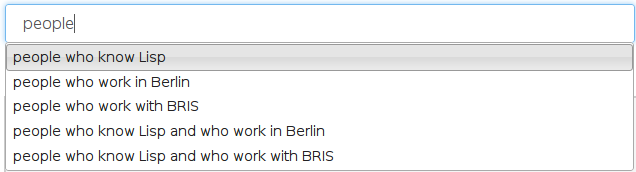
\includegraphics[scale=0.6,keepaspectratio,valign=t]{./gfx/people.png}
\caption{Suggestions based on the word \texttt{people} by using EnglishRGL or EnglishConcat\label{fig:suggestions-people}}
\end{figure}

\autoref{fig:suggestions-who-know} shows that it is possible to use a combination of words to retrieve suggestions. It also demonstrates that the words do not have to be the first words in an instruction.

\begin{figure}[H]
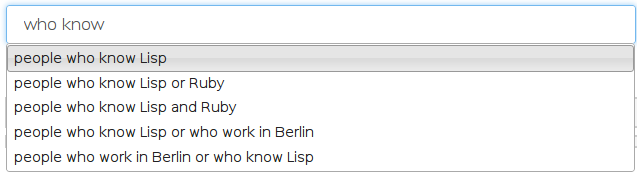
\includegraphics[scale=0.6,keepaspectratio,valign=t]{./gfx/who_know.png}
\caption{Suggestions based on the words \texttt{who know} by using EnglishRGL or EnglishConcat\label{fig:suggestions-who-know}}
\end{figure}

The next four figures shows how it is possible to retreive suggestions based on only names.

\begin{figure}[H]
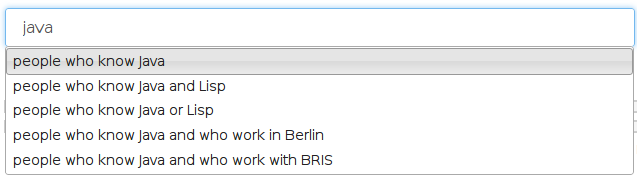
\includegraphics[scale=0.6,keepaspectratio,valign=t]{./gfx/java.png}
\caption{Suggestions based on a name of type Skill by using EnglishRGL or EnglishConcat\label{fig:name-skill}}
\end{figure}

\begin{figure}[H]
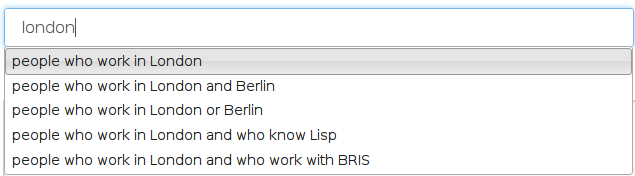
\includegraphics[scale=0.6,keepaspectratio,valign=t]{./gfx/london.png}
\caption{Suggestions based on a name of type Location by using EnglishRGL or EnglishConcat\label{fig:name-location}}
\end{figure}

\begin{figure}[H]
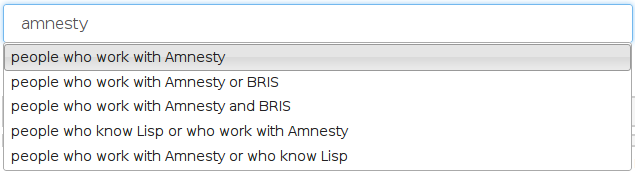
\includegraphics[scale=0.6,keepaspectratio,valign=t]{./gfx/amnesty.png}
\caption{Suggestions based on a name of type Organization by using EnglishRGL or EnglishConcat\label{fig:name-organization}}
\end{figure}

\begin{figure}[H]
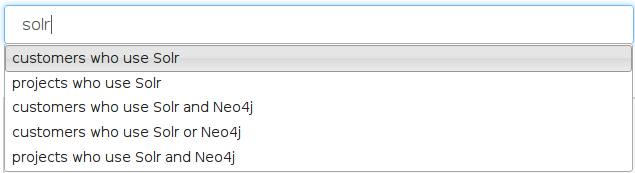
\includegraphics[scale=0.6,keepaspectratio,valign=t]{./gfx/solr.png}
\caption{Suggestions based on a name of type Module by using EnglishRGL or EnglishConcat\label{fig:name-module}}
\end{figure}

\autoref{fig:java-python} shows suggestions based on two names of the same type.

\begin{figure}[H]
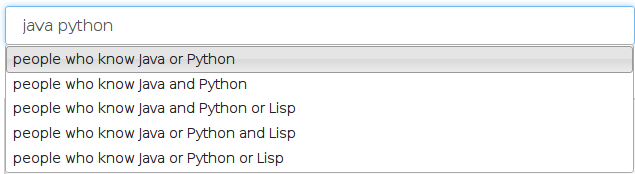
\includegraphics[scale=0.6,keepaspectratio,valign=t]{./gfx/java_python.png}
\caption{Suggestions based on two names  of type Skill by using EnglishRGL or EnglishConcat\label{fig:java-python}}
\end{figure}

\autoref{fig:haskell-london} shows that names do not have to be of the same type to suggest relevant instructions.

\begin{figure}[H]
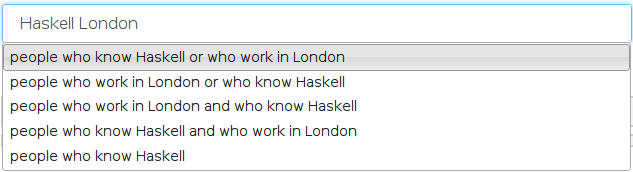
\includegraphics[scale=0.6,keepaspectratio,valign=t]{./gfx/haskell-london.png}
\caption{Suggestions based on two names of different types by using EnglishRGL or EnglishConcat\label{fig:haskell-london}}
\end{figure}

\autoref{fig:persons} shows how we can use the word \texttt{persons} in order to get suggestions. The word \texttt{persons} does not exist in any suggestion, but as it is a synonym to \texttt{people}, the application suggest relevant instructions.

\begin{figure}[H]
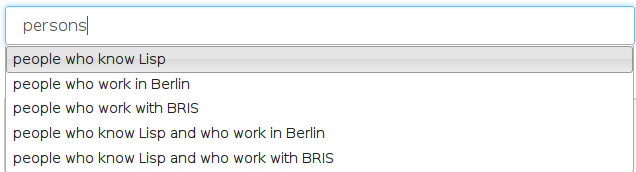
\includegraphics[scale=0.6,keepaspectratio,valign=t]{./gfx/persons.png}
\caption{Synonyms based on a synonym by using EnglishRGL or EnglishConcat\label{fig:persons}}
\end{figure}

Also \autoref{fig:that} shows how we can get suggestions based on a synonym. However, only EnglishConcat gives suggestions based on the word \emph{that}.

\begin{figure}[H]
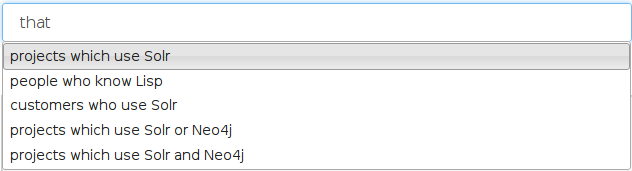
\includegraphics[scale=0.6,keepaspectratio,valign=t]{./gfx/that.png}
\caption{Synonyms based on a synonym by using EnglishConcat\label{fig:that}}
\end{figure}

\autoref{fig:misspelled-name} shows how the application shows relevant suggestion based on a misspelled word.

\begin{figure}[H]
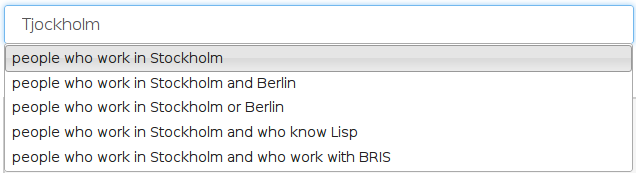
\includegraphics[scale=0.6,keepaspectratio,valign=t]{./gfx/misspelled_name.png}
\caption{Suggestions based on a misspelled word by using EnglishRGL or EnglishConcat\label{fig:misspelled-name}}
\end{figure}

\autoref{fig:projects-rgl} and \autoref{fig:projects-concat} show how the same word can obtain different suggestions by using the concrete languages EnglishRGL and EnglishConcat.

\begin{figure}[H]
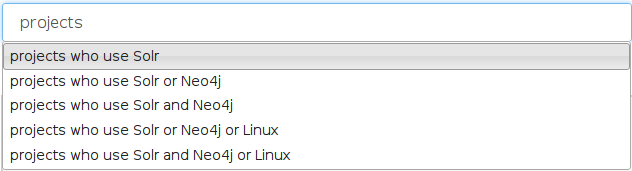
\includegraphics[scale=0.6,keepaspectratio,valign=t]{./gfx/projects-rgl.png}
\caption{Suggestions based on the string \emph{projects} by using EnglishRGL\label{fig:projects-rgl}}
\end{figure}

\begin{figure}[H]
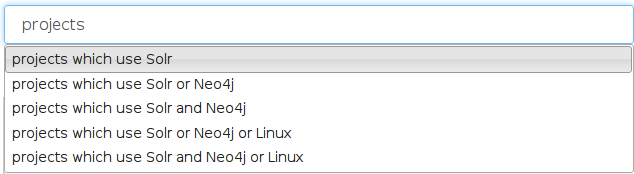
\includegraphics[scale=0.6,keepaspectratio,valign=t]{./gfx/projects-concat.png}
\caption{Suggestions based on the string \emph{projects} by using EnglishConcat\label{fig:projects-concat}}
\end{figure}

Lastly, \autoref{fig:swedish} demonstrates that the application also can translate give suggestions in Swedish. The application can translate valid Swedish sentences as long as the user has chosen Swedish as input language in the application. All instructions that can be translated from English can also be translated from Swedish.

\begin{figure}[H]
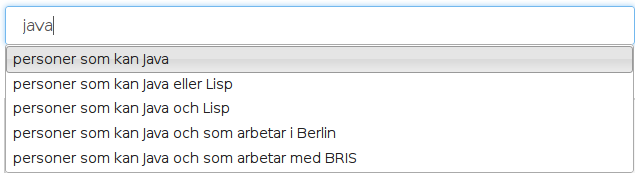
\includegraphics[scale=0.6,keepaspectratio,valign=t]{./gfx/swedish.png}
\caption{Suggestions in Swedish by using SwedishRGL\label{fig:swedish}}
\end{figure}
%************************************************
\chapter{Results}\label{ch:results}
%************************************************
This chapter presents results from the end application.

\section{Translations}
We begin by demonstrating how a few sentences are parsed into an abstract syntax which is linearized into all possible concrete syntaxes. The input is shown in the first box in each figure (with input language as a comment) and the result in second (larger) box. The result of a translation is JSON-data, given by the application.

The first five figures shows the most simplest translations. They include all subjects and all types of names. Each one contains a subject, one verb and one name of a certain type.
\newline
\newline

\autoref{fig:result1} shows that the word \texttt{Java} is of the type \texttt{Skill}.

\begin{figure}[H]
\begin{terminal}
-- EnglishRGL
people who know Java
\end{terminal}
\begin{json-small}
[
 {
  'ast': 'InstrucInternal People (Know_R (MkSkill (MkSymb "Java")))',
  'linearizations': [
   {
    'query': 'people who know Java',
    'language': 'InstrucsEngConcat'
   },
   {
    'query': 'people who know Java',
    'language': 'InstrucsEngRGL'
   },
   {
    'query': 'select?q=*:*&wt=json&fq= object_type : Person AND KNOWS : ( Java )',
    'language': 'InstrucsSolr'
   },
   {
    'query': 'personer som kan Java',
    'language': 'InstrucsSweRGL'
   }
  ]
 }
]
\end{json-small}
\caption{Translation including \texttt{people} and a name of type \texttt{Skill}\label{fig:result1}}
\end{figure}

\autoref{fig:result2} shows that the word \texttt{London} is of the type \texttt{Location}.

\begin{figure}[H]
\begin{terminal}
-- English RGL
people who work in London
\end{terminal}
\begin{json-small}
[
 {
  'ast': 'InstrucInternal People (WorkIn_R (MkLocation (MkSymb "London")))',
  'linearizations': [
   {
    'query': 'people who work in London',
    'language': 'InstrucsEngConcat'
   },
   {
    'query': 'people who work in London',
    'language': 'InstrucsEngRGL'
   },
   {
    'query': 'select?q=*:*&wt=json&fq= object_type : Person AND WORKS_IN : ( London )',
    'language': 'InstrucsSolr'
   },
   {
    'query': 'personer som arbetar i London',
    'language': 'InstrucsSweRGL'
   }
  ]
 }
]
\end{json-small}
\caption{Translation including \texttt{people} and a name of type \texttt{Location}\label{fig:result2}}
\end{figure}

\autoref{fig:result3} shows that the word \texttt{Amnesty} is of the type \texttt{Organization}.

\begin{figure}[H]
\begin{terminal}
-- EnglishRGL
people who work with Amnesty
\end{terminal}
\begin{json-small}
[
 {
  'ast': 'InstrucInternal People (WorkWith_R (MkOrganization (MkSymb "Amnesty")))',
  'linearizations': [
   {
    'query': 'people who work with Amnesty',
    'language': 'InstrucsEngConcat'
   },
   {
    'query': 'people who work with Amnesty',
    'language': 'InstrucsEngRGL'
   },
   {
    'query': 'select?q=*:*&wt=json&fq= object_type : Person AND WORKS_WITH : ( Amnesty )',
    'language': 'InstrucsSolr'
   },
   {
    'query': 'personer som arbetar med Amnesty',
    'language': 'InstrucsSwe'
   }
  ]
 }
]
\end{json-small}
\caption{Translation including \texttt{people} and a name of type \texttt{Organization}\label{fig:result3}}
\end{figure}

\autoref{fig:result4} shows that the word \texttt{Solr} is of the type \texttt{Module}.

\begin{figure}[H]
\begin{terminal}
-- EnglishRGL
customers who use Solr
\end{terminal}
\begin{json-small}
[
 {
  'ast': 'InstrucExternal Customer (UseExt_R (MkModule (MkSymb "Solr")))',
  'linearizations': [
   {
    'query': 'customers who use Solr',
    'language': 'InstrucsEngConcat'
   },
   {
    'query': 'customers who use Solr',
    'language': 'InstrucsEngRGL'
   },
   {
    'query': 'select?q=*:*&wt=json&fq= object_type : Organization AND USES : ( Solr )',
    'language': 'InstrucsSolr'
   },
   {
    'query': 'kunder som använder Solr',
    'language': 'InstrucsSwe'
   }
  ]
 }
]
\end{json-small}
\caption{Translation including \texttt{customer} and a name of type \texttt{Module}\label{fig:result4}}
\end{figure}

Similarly, also \autoref{fig:result5} shows that the word \texttt{Solr} is of the type \texttt{Module}.

\begin{figure}[H]
\begin{terminal}
-- EnglishRGL
projects who use Solr
\end{terminal}
\begin{json-small}
[
 {
  'ast': 'InstrucResource Project (UseRes_R (MkModule (MkSymb "Solr")))',
  'linearizations': [
   {
    'query': 'projects who use Solr',
    'language': 'InstrucsEngConcat'
   },
   {
    'query': 'projects who use Solr',
    'language': 'InstrucsEngRGL'
   },
   {
    'query': 'select?q=*:*&wt=json&fq= object_type : Project AND USES : ( Solr )',
    'language': 'InstrucsSolr'
   },
   {
    'query': 'projekt som använder Solr',
    'language': 'InstrucsSwe'
   }
  ]
 }
]
\end{json-small}
\caption{Translation including \texttt{project} and a name of type \texttt{Module}\label{fig:result5}}
\end{figure}

\autoref{fig:translation-java-python} shows how the applications handles the boolean operator \emph{and}. The application handles the case for \emph{or} similarly.

\begin{figure}[H]
\begin{terminal}
-- EnglishRGL
people who know Java and Python
\end{terminal}
\begin{json-small}
[
 {
  'ast': 'InstrucInternal People (Know_R (And_S (MkSkill (MkSymb "Java")) 
                                                      (MkSkill (MkSymb "Python"))))',
  'linearizations': [
   {
    'query': 'people who know Java and Python',
    'language': 'InstrucsEngConcat'
   },
   {
    'query': 'people who know Java and Python',
    'language': 'InstrucsEngRGL'
   },
   {
    'query': 'select?q=*:*&wt=json&fq= object_type : Person AND 
                                                KNOWS : ( ( Java ) AND ( Python ) )',
    'language': 'InstrucsSolr'
   },
   {
    'query': 'personer som kan Java och Python',
    'language': 'InstrucsSwe'
   }
  ]
 }
]
\end{json-small}
\caption{Translation including \texttt{people} and two names of the type \texttt{Skill}\label{fig:translation-java-python}}
\end{figure}

\autoref{fig:translation-ambig} shows how the application handles an ambiguous instruction. Two abstract syntax trees are seen in the result, as there are two ways of interpreting the instruction. The different interpretations can be modelled as follows: \emph{people who know (Java and Python) or Haskell} or \emph{people who know Java and (Python or Haskell)}.

\begin{figure}[H]
\begin{terminal}
-- EnglishRGL
people who know Java and Python or Haskell
\end{terminal}
\begin{json-small}
[
 {
  'ast': 'InstrucInternal People (Know_R (Or_S (And_S (MkSkill (MkSymb "Java")) 
                       (MkSkill (MkSymb "Python"))) (MkSkill (MkSymb "Haskell"))))',
  'linearizations': [
   {
    'query': 'people who know Java and Python or Haskell',
    'language': 'InstrucsEngConcat'
   },
   {
    'query': 'people who know Java and Python or Haskell',
    'language': 'InstrucsEngRGL'
   },
   {
    'query': 'select?q=*:*&wt=json&fq= object_type : Person AND 
                      KNOWS : ( ( ( Java ) AND ( Python ) ) OR ( Haskell ) )',
    'language': 'InstrucsSolr'
   },
   {
    'query': 'personer som kan Java och Python eller Haskell',
    'language': 'InstrucsSwe'
   }
  ]
 },
 {
  'ast': 'InstrucInternal People (Know_R (And_S (MkSkill (MkSymb "Java")) 
                      (Or_S (MkSkill (MkSymb "Python")) (MkSkill (MkSymb "Haskell")))))',
  'linearizations': [
   {
    'query': 'people who know Java and Python or Haskell',
    'language': 'InstrucsEngConcat'
   },
   {
    'query': 'people who know Java and Python or Haskell',
    'language': 'InstrucsEngRGL'
   },
   {
    'query': 'select?q=*:*&wt=json&fq= object_type : Person AND 
                      KNOWS : ( ( Java ) AND ( ( Python ) OR ( Haskell ) ) )',
    'language': 'InstrucsSolr'
   },
   {
    'query': 'personer som kan Java och Python eller Haskell',
    'language': 'InstrucsSwe'
   }
  ]
 }
]
\end{json-small}
\caption{Translation of an ambiguous instruction involving \texttt{people} and three names of the type \texttt{Skill}\label{fig:translation-ambig}}
\end{figure}

\section{Suggestions}
This section shows how the application reacts to input before the user has chosen to translate the instruction. Each figure shows an image of how the application suggest valid sentences from a partial instruction.

\autoref{fig:suggestions-people} shows suggestions based on the first word in a valid sentence.

\begin{figure}[H]
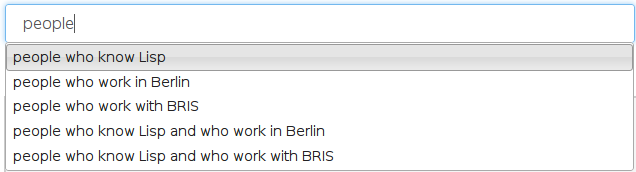
\includegraphics[scale=0.6,keepaspectratio,valign=t]{./gfx/people.png}
\caption{Suggestions based on the word \texttt{people} by using EnglishRGL or EnglishConcat\label{fig:suggestions-people}}
\end{figure}

\autoref{fig:suggestions-who-know} shows that it is possible to use a combination of words to retrieve suggestions. It also demonstrates that the words do not have to be the first words in an instruction.

\begin{figure}[H]
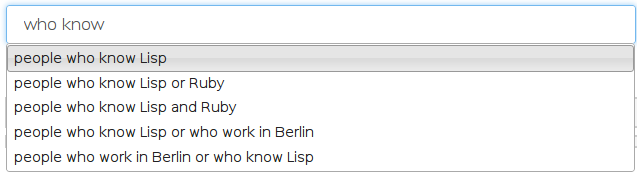
\includegraphics[scale=0.6,keepaspectratio,valign=t]{./gfx/who_know.png}
\caption{Suggestions based on the words \texttt{who know} by using EnglishRGL or EnglishConcat\label{fig:suggestions-who-know}}
\end{figure}

The next four figures shows how it is possible to retreive suggestions based on only names.

\begin{figure}[H]
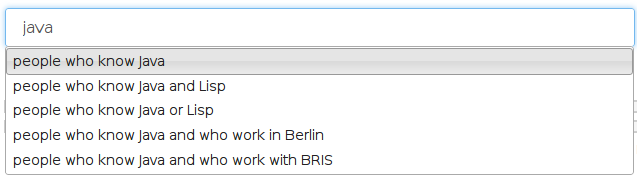
\includegraphics[scale=0.6,keepaspectratio,valign=t]{./gfx/java.png}
\caption{Suggestions based on a name of type Skill by using EnglishRGL or EnglishConcat\label{fig:name-skill}}
\end{figure}

\begin{figure}[H]
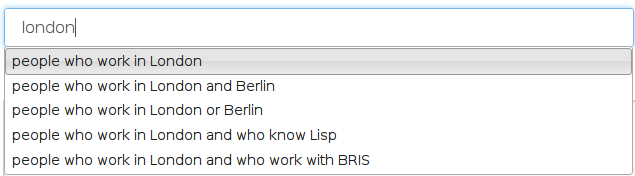
\includegraphics[scale=0.6,keepaspectratio,valign=t]{./gfx/london.png}
\caption{Suggestions based on a name of type Location by using EnglishRGL or EnglishConcat\label{fig:name-location}}
\end{figure}

\begin{figure}[H]
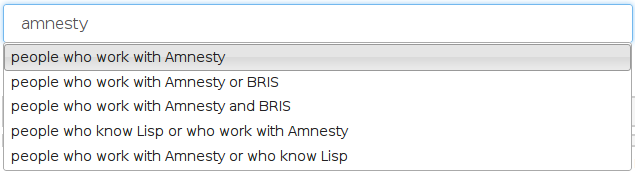
\includegraphics[scale=0.6,keepaspectratio,valign=t]{./gfx/amnesty.png}
\caption{Suggestions based on a name of type Organization by using EnglishRGL or EnglishConcat\label{fig:name-organization}}
\end{figure}

\begin{figure}[H]
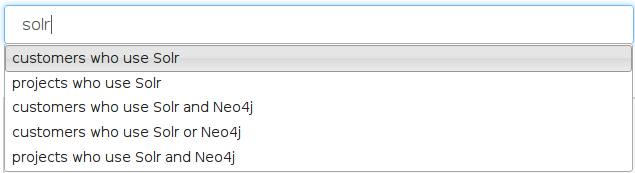
\includegraphics[scale=0.6,keepaspectratio,valign=t]{./gfx/solr.png}
\caption{Suggestions based on a name of type Module by using EnglishRGL or EnglishConcat\label{fig:name-module}}
\end{figure}

\autoref{fig:java-python} shows suggestions based on two names of the same type.

\begin{figure}[H]
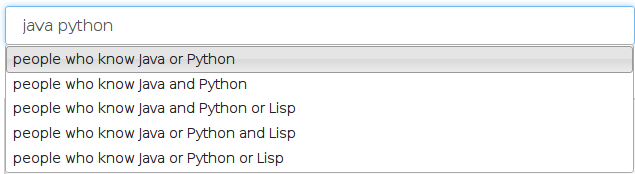
\includegraphics[scale=0.6,keepaspectratio,valign=t]{./gfx/java_python.png}
\caption{Suggestions based on two names  of type Skill by using EnglishRGL or EnglishConcat\label{fig:java-python}}
\end{figure}

\autoref{fig:haskell-london} shows that names do not have to be of the same type to suggest relevant instructions.

\begin{figure}[H]
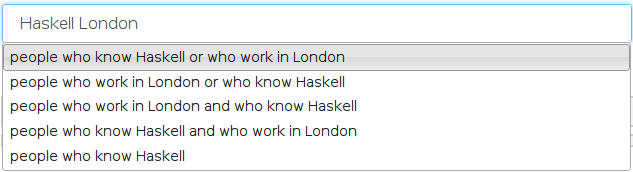
\includegraphics[scale=0.6,keepaspectratio,valign=t]{./gfx/haskell-london.png}
\caption{Suggestions based on two names of different types by using EnglishRGL or EnglishConcat\label{fig:haskell-london}}
\end{figure}

\autoref{fig:persons} shows how we can use the word \texttt{persons} in order to get suggestions. The word \texttt{persons} does not exist in any suggestion, but as it is a synonym to \texttt{people}, the application suggest relevant instructions.

\begin{figure}[H]
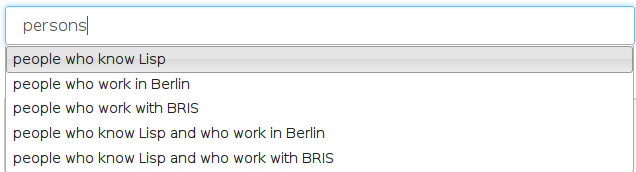
\includegraphics[scale=0.6,keepaspectratio,valign=t]{./gfx/persons.png}
\caption{Synonyms based on a synonym by using EnglishRGL or EnglishConcat\label{fig:persons}}
\end{figure}

Also \autoref{fig:that} shows how we can get suggestions based on a synonym. Both EnglishRGL and EnglishConcat gives suggestions based on the word \emph{that}.

\begin{figure}[H]
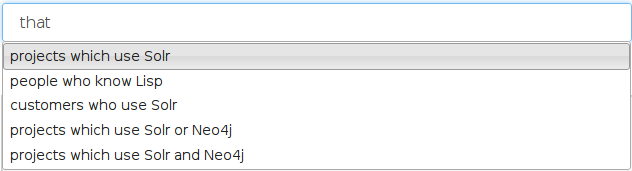
\includegraphics[scale=0.6,keepaspectratio,valign=t]{./gfx/that.png}
\caption{Synonyms based on a synonym by using EnglishConcat\label{fig:that}}
\end{figure}

\autoref{fig:misspelled-name} shows how the application shows relevant suggestion based on a misspelled word.

\begin{figure}[H]
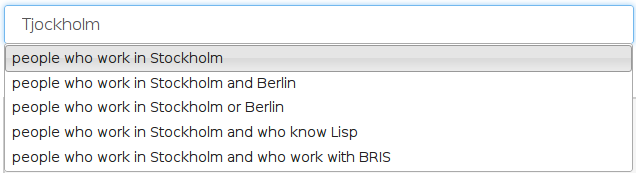
\includegraphics[scale=0.6,keepaspectratio,valign=t]{./gfx/misspelled_name.png}
\caption{Suggestions based on a misspelled word by using EnglishRGL or EnglishConcat\label{fig:misspelled-name}}
\end{figure}

\autoref{fig:projects-rgl} and \autoref{fig:projects-concat} show how the same word can obtain different suggestions by using the concrete languages EnglishRGL and EnglishConcat.

\begin{figure}[H]
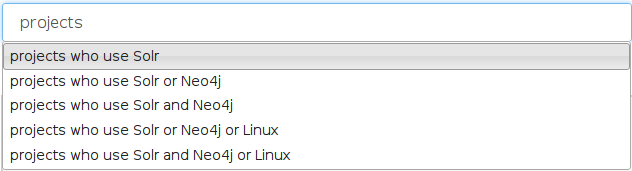
\includegraphics[scale=0.6,keepaspectratio,valign=t]{./gfx/projects-rgl.png}
\caption{Suggestions based on the string \emph{projects} by using EnglishRGL\label{fig:projects-rgl}}
\end{figure}

\begin{figure}[H]
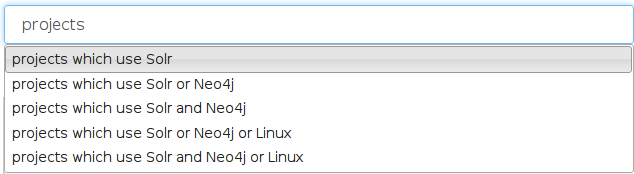
\includegraphics[scale=0.6,keepaspectratio,valign=t]{./gfx/projects-concat.png}
\caption{Suggestions based on the string \emph{projects} by using EnglishConcat\label{fig:projects-concat}}
\end{figure}

Lastly, \autoref{fig:swedish} demonstrates that the application also can translate give suggestions in Swedish. The application can translate valid Swedish sentences as long as the user has chosen SwedishRGL as input language in the application. All instructions that can be translated from EnglishRGL can also be translated from SwedishRGL.

\begin{figure}[H]
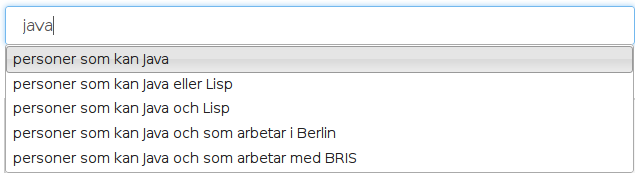
\includegraphics[scale=0.6,keepaspectratio,valign=t]{./gfx/swedish.png}
\caption{Suggestions in Swedish by using SwedishRGL\label{fig:swedish}}
\end{figure}
%************************************************
\chapter{Discussion}\label{ch:discussion}
%************************************************

\section{Contributions}
My work has improved PGF, at least a bit


Issue with the suggestion algorithm, cannot take more than one word..
%\addtocontents{toc}{\protect\clearpage} % <--- just debug stuff, ignore
%%************************************************
\chapter{Results}\label{ch:results}
%************************************************
This chapter presents results from the end application.

\section{Translation}
We begin by demonstrating how a few sentences are parsed into an abstract syntax which is linearized into all possible concrete syntaxes. The input is shown in the first box in each figure (with input language as a comment) and the result in second (larger) box. The result of a translation is JSON-data, given by the application.

The first five figures shows the most simplest translations. They include all subjects and all types of names. Each one contains a subject, one verb and one name of a certain type.

\begin{figure}[H]
\begin{terminal}
-- EnglishRGL
people who know Java
\end{terminal}
\begin{json-small}
[
 {
  'ast': 'InstrucInternal People (Know_R (MkSkill (MkSymb "Java")))',
  'linearizations': [
   {
    'query': 'people who know Java',
    'language': 'InstrucsEngConcat'
   },
   {
    'query': 'people who know Java',
    'language': 'InstrucsEngRGL'
   },
   {
    'query': 'select?q=*:*&wt=json&fq= object_type : Person AND KNOWS : ( Java )',
    'language': 'InstrucsSolr'
   },
   {
    'query': 'personer som kan Java',
    'language': 'InstrucsSweRGL'
   }
  ]
 }
]
\end{json-small}
\caption{Translation including \texttt{people} and a name of type \texttt{Skill}\label{fig:asts-depths}}
\end{figure}

\begin{figure}[H]
\begin{terminal}
-- English RGL
people who work in London
\end{terminal}
\begin{json-small}
[
 {
  'ast': 'InstrucInternal People (WorkIn_R (MkLocation (MkSymb "London")))',
  'linearizations': [
   {
    'query': 'people who work in London',
    'language': 'InstrucsEngConcat'
   },
   {
    'query': 'people who work in London',
    'language': 'InstrucsEngRGL'
   },
   {
    'query': 'select?q=*:*&wt=json&fq= object_type : Person AND WORKS_IN : ( London )',
    'language': 'InstrucsSolr'
   },
   {
    'query': 'personer som arbetar i London',
    'language': 'InstrucsSweRGL'
   }
  ]
 }
]
\end{json-small}
\caption{Translation including \texttt{people} and a name of type \texttt{Location}\label{fig:asts-depths}}
\end{figure}

\begin{figure}[H]
\begin{terminal}
-- EnglishRGL
people who work with Amnesty
\end{terminal}
\begin{json-small}
[
 {
  'ast': 'InstrucInternal People (WorkWith_R (MkOrganization (MkSymb "Amnesty")))',
  'linearizations': [
   {
    'query': 'people who work with Amnesty',
    'language': 'InstrucsEngConcat'
   },
   {
    'query': 'people who work with Amnesty',
    'language': 'InstrucsEngRGL'
   },
   {
    'query': 'select?q=*:*&wt=json&fq= object_type : Person AND WORKS_WITH : ( Amnesty )',
    'language': 'InstrucsSolr'
   },
   {
    'query': 'personer som arbetar med Amnesty',
    'language': 'InstrucsSwe'
   }
  ]
 }
]
\end{json-small}
\caption{Translation including \texttt{people} and a name of type \texttt{Organization}\label{fig:asts-depths}}
\end{figure}

\begin{figure}[H]
\begin{terminal}
-- EnglishRGL
customers who use Solr
\end{terminal}
\begin{json-small}
[
 {
  'ast': 'InstrucExternal Customer (UseExt_R (MkModule (MkSymb "Solr")))',
  'linearizations': [
   {
    'query': 'customers who use Solr',
    'language': 'InstrucsEngConcat'
   },
   {
    'query': 'customers who use Solr',
    'language': 'InstrucsEngRGL'
   },
   {
    'query': 'select?q=*:*&wt=json&fq= object_type : Organization AND USES : ( Solr )',
    'language': 'InstrucsSolr'
   },
   {
    'query': 'kunder som använder Solr',
    'language': 'InstrucsSwe'
   }
  ]
 }
]
\end{json-small}
\caption{Translation including \texttt{customer} and a name of type \texttt{Module}\label{fig:asts-depths}}
\end{figure}

\begin{figure}[H]
\begin{terminal}
-- EnglishRGL
projects who use Solr
\end{terminal}
\begin{json-small}
[
 {
  'ast': 'InstrucResource Project (UseRes_R (MkModule (MkSymb "Solr")))',
  'linearizations': [
   {
    'query': 'projects who use Solr',
    'language': 'InstrucsEngConcat'
   },
   {
    'query': 'projects who use Solr',
    'language': 'InstrucsEngRGL'
   },
   {
    'query': 'select?q=*:*&wt=json&fq= object_type : Project AND USES : ( Solr )',
    'language': 'InstrucsSolr'
   },
   {
    'query': 'projekt som använder Solr',
    'language': 'InstrucsSwe'
   }
  ]
 }
]
\end{json-small}
\caption{Translation including \texttt{project} and a name of type \texttt{Module}\label{fig:asts-depths}}
\end{figure}

\autoref{fig:translation-java-python} shows how the applications handles the boolean operator \emph{and}. The application handles the case for \emph{or} similarly.

\begin{figure}[H]
\begin{terminal}
-- EnglishRGL
people who know Java and Python
\end{terminal}
\begin{json-small}
[
 {
  'ast': 'InstrucInternal People (Know_R (And_S (MkSkill (MkSymb "Java")) 
                                                      (MkSkill (MkSymb "Python"))))',
  'linearizations': [
   {
    'query': 'people who know Java and Python',
    'language': 'InstrucsEngConcat'
   },
   {
    'query': 'people who know Java and Python',
    'language': 'InstrucsEngRGL'
   },
   {
    'query': 'select?q=*:*&wt=json&fq= object_type : Person AND 
                                                KNOWS : ( ( Java ) AND ( Python ) )',
    'language': 'InstrucsSolr'
   },
   {
    'query': 'personer som kan Java och Python',
    'language': 'InstrucsSwe'
   }
  ]
 }
]
\end{json-small}
\caption{Translation including \texttt{people} and two names of the type \texttt{Skill}\label{fig:translation-java-python}}
\end{figure}

\newpage

\autoref{fig:translation-ambig} shows how the application handles an ambiguous instruction. Two abstract syntax trees are seen in the result, as there are two ways of interpreting the instruction. The different interpretations can be modelled as follows: \emph{people who know (Java and Python) or Haskell} or \emph{people who know Java and (Python or Haskell)}.

\begin{figure}[H]
\begin{terminal}
-- EnglishRGL
people who know Java and Python or Haskell
\end{terminal}
\begin{json-small}
[
 {
  'ast': 'InstrucInternal People (Know_R (Or_S (And_S (MkSkill (MkSymb "Java")) 
                       (MkSkill (MkSymb "Python"))) (MkSkill (MkSymb "Haskell"))))',
  'linearizations': [
   {
    'query': 'people who know Java and Python or Haskell',
    'language': 'InstrucsEngConcat'
   },
   {
    'query': 'people who know Java and Python or Haskell',
    'language': 'InstrucsEngRGL'
   },
   {
    'query': 'select?q=*:*&wt=json&fq= object_type : Person AND 
                      KNOWS : ( ( ( Java ) AND ( Python ) ) OR ( Haskell ) )',
    'language': 'InstrucsSolr'
   },
   {
    'query': 'personer som kan Java och Python eller Haskell',
    'language': 'InstrucsSwe'
   }
  ]
 },
 {
  'ast': 'InstrucInternal People (Know_R (And_S (MkSkill (MkSymb "Java")) 
                      (Or_S (MkSkill (MkSymb "Python")) (MkSkill (MkSymb "Haskell")))))',
  'linearizations': [
   {
    'query': 'people who know Java and Python or Haskell',
    'language': 'InstrucsEngConcat'
   },
   {
    'query': 'people who know Java and Python or Haskell',
    'language': 'InstrucsEngRGL'
   },
   {
    'query': 'select?q=*:*&wt=json&fq= object_type : Person AND 
                      KNOWS : ( ( Java ) AND ( ( Python ) OR ( Haskell ) ) )',
    'language': 'InstrucsSolr'
   },
   {
    'query': 'personer som kan Java och Python eller Haskell',
    'language': 'InstrucsSwe'
   }
  ]
 }
]
\end{json-small}
\caption{Translation of an ambiguous instruction involving \texttt{people} and three names of the type \texttt{Skill}\label{fig:translation-ambig}}
\end{figure}

\section{Suggestions}
This section shows how the application reacts to input before the user has chosen to translate the instruction. Each figure shows an image of how the application suggest valid sentences from a partial instruction.

\autoref{fig:suggestions-people} shows suggestions based on the first word in a valid sentence.

\begin{figure}[H]
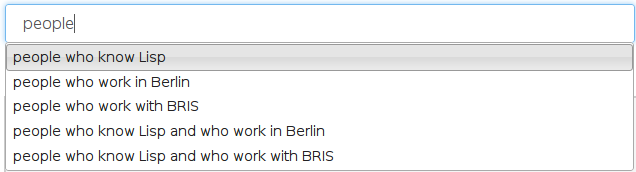
\includegraphics[scale=0.6,keepaspectratio,valign=t]{./gfx/people.png}
\caption{Suggestions based on the word \texttt{people} by using EnglishRGL or EnglishConcat\label{fig:suggestions-people}}
\end{figure}

\autoref{fig:suggestions-who-know} shows that it is possible to use a combination of words to retrieve suggestions. It also demonstrates that the words do not have to be the first words in an instruction.

\begin{figure}[H]
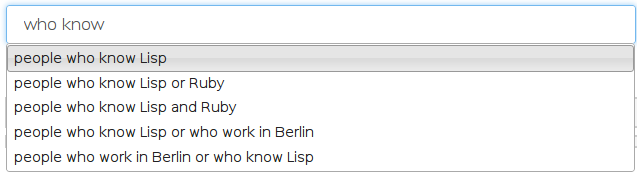
\includegraphics[scale=0.6,keepaspectratio,valign=t]{./gfx/who_know.png}
\caption{Suggestions based on the words \texttt{who know} by using EnglishRGL or EnglishConcat\label{fig:suggestions-who-know}}
\end{figure}

The next four figures shows how it is possible to retreive suggestions based on only names.

\begin{figure}[H]
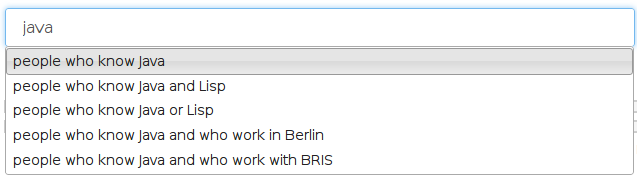
\includegraphics[scale=0.6,keepaspectratio,valign=t]{./gfx/java.png}
\caption{Suggestions based on a name of type Skill by using EnglishRGL or EnglishConcat\label{fig:name-skill}}
\end{figure}

\begin{figure}[H]
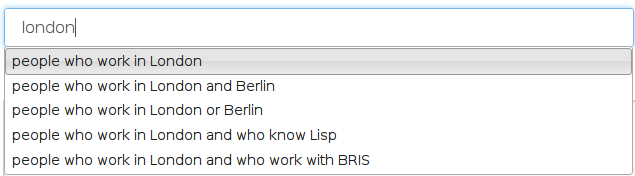
\includegraphics[scale=0.6,keepaspectratio,valign=t]{./gfx/london.png}
\caption{Suggestions based on a name of type Location by using EnglishRGL or EnglishConcat\label{fig:name-location}}
\end{figure}

\begin{figure}[H]
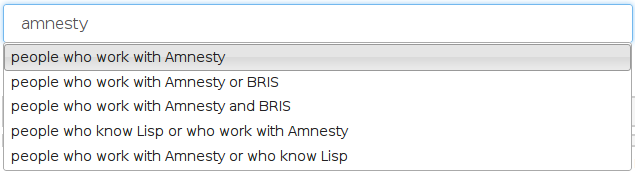
\includegraphics[scale=0.6,keepaspectratio,valign=t]{./gfx/amnesty.png}
\caption{Suggestions based on a name of type Organization by using EnglishRGL or EnglishConcat\label{fig:name-organization}}
\end{figure}

\begin{figure}[H]
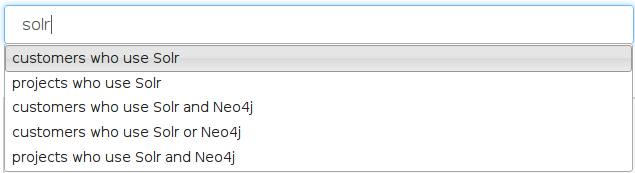
\includegraphics[scale=0.6,keepaspectratio,valign=t]{./gfx/solr.png}
\caption{Suggestions based on a name of type Module by using EnglishRGL or EnglishConcat\label{fig:name-module}}
\end{figure}

\autoref{fig:java-python} shows suggestions based on two names of the same type.

\begin{figure}[H]
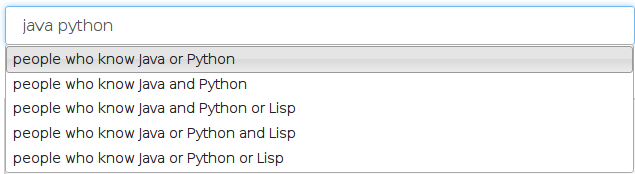
\includegraphics[scale=0.6,keepaspectratio,valign=t]{./gfx/java_python.png}
\caption{Suggestions based on two names  of type Skill by using EnglishRGL or EnglishConcat\label{fig:java-python}}
\end{figure}

\autoref{fig:haskell-london} shows that names do not have to be of the same type to suggest relevant instructions.

\begin{figure}[H]
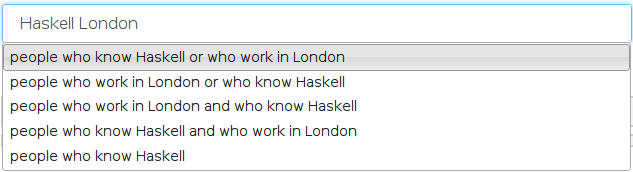
\includegraphics[scale=0.6,keepaspectratio,valign=t]{./gfx/haskell-london.png}
\caption{Suggestions based on two names of different types by using EnglishRGL or EnglishConcat\label{fig:haskell-london}}
\end{figure}

\autoref{fig:persons} shows how we can use the word \texttt{persons} in order to get suggestions. The word \texttt{persons} does not exist in any suggestion, but as it is a synonym to \texttt{people}, the application suggest relevant instructions.

\begin{figure}[H]
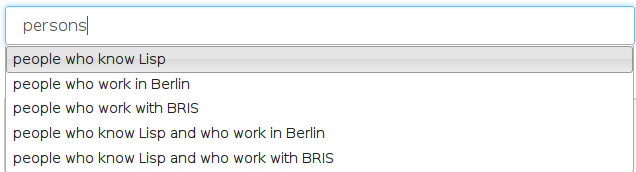
\includegraphics[scale=0.6,keepaspectratio,valign=t]{./gfx/persons.png}
\caption{Synonyms based on a synonym by using EnglishRGL or EnglishConcat\label{fig:persons}}
\end{figure}

Also \autoref{fig:that} shows how we can get suggestions based on a synonym. However, only EnglishConcat gives suggestions based on the word \emph{that}.

\begin{figure}[H]
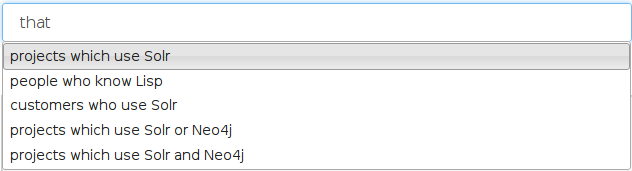
\includegraphics[scale=0.6,keepaspectratio,valign=t]{./gfx/that.png}
\caption{Synonyms based on a synonym by using EnglishConcat\label{fig:that}}
\end{figure}

\autoref{fig:misspelled-name} shows how the application shows relevant suggestion based on a misspelled word.

\begin{figure}[H]
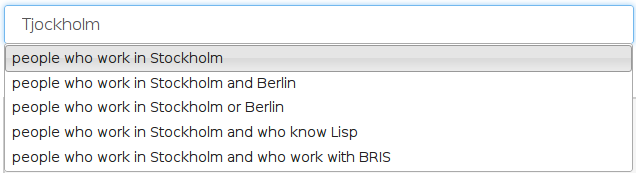
\includegraphics[scale=0.6,keepaspectratio,valign=t]{./gfx/misspelled_name.png}
\caption{Suggestions based on a misspelled word by using EnglishRGL or EnglishConcat\label{fig:misspelled-name}}
\end{figure}

\autoref{fig:projects-rgl} and \autoref{fig:projects-concat} show how the same word can obtain different suggestions by using the concrete languages EnglishRGL and EnglishConcat.

\begin{figure}[H]
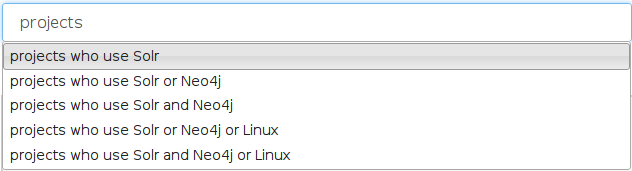
\includegraphics[scale=0.6,keepaspectratio,valign=t]{./gfx/projects-rgl.png}
\caption{Suggestions based on the string \emph{projects} by using EnglishRGL\label{fig:projects-rgl}}
\end{figure}

\begin{figure}[H]
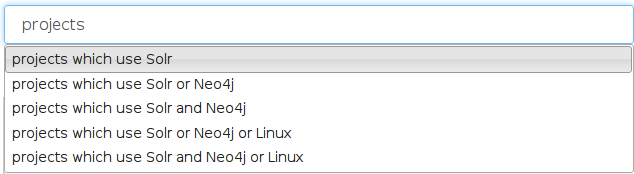
\includegraphics[scale=0.6,keepaspectratio,valign=t]{./gfx/projects-concat.png}
\caption{Suggestions based on the string \emph{projects} by using EnglishConcat\label{fig:projects-concat}}
\end{figure}

Lastly, \autoref{fig:swedish} demonstrates that the application also can translate give suggestions in Swedish. The application can translate valid Swedish sentences as long as the user has chosen Swedish as input language in the application. All instructions that can be translated from English can also be translated from Swedish.

\begin{figure}[H]
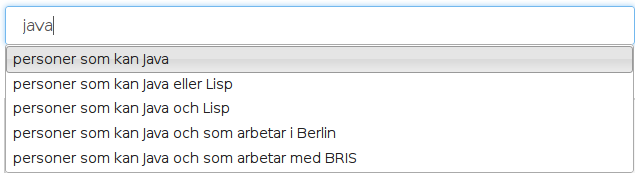
\includegraphics[scale=0.6,keepaspectratio,valign=t]{./gfx/swedish.png}
\caption{Suggestions in Swedish by using SwedishRGL\label{fig:swedish}}
\end{figure}
%\include{multiToC} % <--- just debug stuff, ignore for your documents
% ********************************************************************
% Backmatter
%*******************************************************
\appendix
\cleardoublepage
%\part{Appendix}
%********************************************************************
% Appendix
%*******************************************************
% If problems with the headers: get headings in appendix etc. right
%\markboth{\spacedlowsmallcaps{Appendix}}{\spacedlowsmallcaps{Appendix}}
\chapter{GF runtime systems and libraries}\label{ch:appendix-a}

\section{GF runtime systems}

While the GF-shell is a powerful tool, it is not very convenient to interact with when programming an application. Luckily, the creators of GF has thought about this and built embeddable runtime systems for a few programming languages \cite[p. 3]{angelov:2011}. These runtime systems makes it possible to interact with a grammar directly through language specific data types. We have chosen to work with the Java-runtime system in this project.

\subsection{Portable Grammar Format}
The GF-shell interacts with grammars by interpreting the GF programming language. This allows us to write our grammars in an simple and convenient syntax. Interpreting the GF programming language directly is however a heavy operation\cite{angelov:2011}[p. 13], especially with larger grammars. This is where the \ac{pgf}\cite{angelov:2011}[p. 14] comes in. PGF is a custom made machine language which is dynamically created by compiling a grammar with GF into a PGF-file. The runtime systems works exclusively with PGF-files.

\subsection{GF libraries}
In order to use the Java-runtime, we first need to generate a few libraries which is used by the runtime system. The Java-runtime system depends on the C-runtime system and a special wrapper between the C- and the Java-runtime. The libraries are platform dependent and at the time of writing, no pre-generated libraries exists. We therefore need to generate the libraries by ourselves. We will start by generating and installing the C-libraries. We will then go through how we can generate the wrapper library.

\subsubsection{Building and installing the C-runtime}
Start by fetching the needed dependencies

\begin{terminal}
sudo apt-get install gcc autoconf libtool
\end{terminal}

Download the latest source code of GF from GitHub.

\begin{terminal}
git clone https://github.com/GrammaticalFramework/GF.git
\end{terminal}

It is also possible to download the project as an archive by visiting the repository url.

You will receive a directory \texttt{GF/}. Change the current working directory to the C-runtime folder.

\begin{terminal}
cd GF/src/runtime/c
\end{terminal}

Generate a configuration file

\begin{terminal}
autoreconf -i
\end{terminal}

Check that all dependencies are met

\begin{terminal}
./configure
\end{terminal}

If there exists a dependency that is not fulfilled, try to install an appropriate package using your package-manager.

Build the program

\begin{terminal}
make
\end{terminal}

Install the libraries you just built

\begin{terminal}
sudo make install
\end{terminal}

The C-runtime for PGF is now installed.

\subsection{Building and installing the C to Java wrapper library}
Start by installing the needed dependency

\begin{terminal}
sudo apt-get install g++
\end{terminal}

The wrapper is built by using a script which is executed in Eclipse. This step assumes that you have Eclipse installed with the CDT-plugin. If you don't have Eclipse, you can download it with your package manager, just do not forget to install the CDT-plugin.

Start Eclipse and choose \texttt{File} > \texttt{Import..} in the menu. Choose \texttt{Import Existing Projects into Workspace} and click on the \texttt{Next} button. Select \texttt{Browse...} and navigate to the location where you downloaded GF from GitHub and press enter. Uncheck everything except \texttt{jpgf} and click on \texttt{Finish}. You have now imported the project which can build the Java-runtime system. 

Unfortunately, the build-configuration for the jpgf-project is not complete at time of writing. We therefore need to make additional adjustments in order to build the project.

Right-click on the project and choose \texttt{Properties}. Click on \texttt{Includes} which is located below \texttt{GCC C Compiler}. You will see one directory listed in the textbox. You need to check that this directory exists. If not, change it to the correct one. For instance, this tutorial was written using Ubuntu 14.04 amd64 with OpenJDK 7, hence the correct directory is

\begin{terminal}
/usr/lib/jvm/java-7-openjdk-amd64/include
\end{terminal}

The project also needs another flag in order to build properly. In the \texttt{Properties}-window, click on \texttt{Miscellaneous} below \texttt{GCC C Compiler}. Add \texttt{-fPIC} to the text field next to \texttt{Other flags}. Click on \texttt{Ok} to save the settings.

You can now build the project by choosing \texttt{Project} > \texttt{Build Project} in the menu. If everything went well you shall have generated a file \texttt{libjpgf.so} in \texttt{Release (posix)/} . You can check that the dependencies of \texttt{libjpgf.so} is fulfilled (i.e. it finds the C-runtime) by executing the following in a terminal

\begin{terminal}
ldd libjpgf.so
\end{terminal}

If you cannot see \texttt{not found} anywhere in the results, all dependencies are met. However if some dependencies are missing, try to locate the files and move them to \texttt{/usr/local/lib} (or \texttt{/usr/lib} in some distros).

The last step is to move \texttt{libjpgf.so} into the correct directory.

\begin{terminal}
mv libjpgf.so /usr/local/lib (or /usr/lib)
\end{terminal}

You have now installed the wrapper library.

\subsection{Using the Java-runtime}
Have not started on this yet...
\todo{Don't forget how to set java lib path when using tomcat!}
%********************************************************************
% Appendix
%*******************************************************
% If problems with the headers: get headings in appendix etc. right
%\markboth{\spacedlowsmallcaps{Appendix}}{\spacedlowsmallcaps{Appendix}}
\chapter{Installing the application}\label{ch:appendix-b}

While \autoref{ch:appendix-a} focused on installing GF-related dependencies, this appendix explains how the application can be installed into an application server. Note that the application will not run unless all GF-dependencies are installed. The application (and the source code) can be downloaded from \href{http://thesis.agfjord.se/}{thesis.agfjord.se} where also a working demo of the application can be found.

\section{Installing and configurating Apache Tomcat}
This application can be executed by using any application server that supports \texttt{WAR}-files. The \texttt{WAR}-file in this project is built using Maven, which can also upload the file to an instance of the application server Tomcat. This method is very convenient since it automates a lot work. The following section describes how to install and configure Tomcat and Maven to work with this project.

Download and install Tomcat 8 and Maven (here by using aptitude package-manager).

\begin{terminal}
$ sudo apt-get install tomcat8 tomcat8-admin maven
\end{terminal}
%$

Tomcat requires an uploader to have the correct permissions.
\newline
Edit \texttt{/etc/tomcat8/tomcat-users.xml} and add the following:

\begin{terminal}
/etc/tomcat8/tomcat-users.xml
------------------------------------------------
<tomcat-users>
  <role rolename="manager-gui"/>
  <role rolename="manager-script"/>
  <user username="admin" password="secr3t" roles="manager-gui,manager-script"/>
</tomcat-users>
\end{terminal}

As the application will use the generated wrapper library \texttt{libjpgf.so}, we need to make a proper reference to this library and its dependencies (the C-libraries). This is achieved by creating a new file \texttt{setenv.sh} in the directory \texttt{/usr/share/tomcat8/bin/}, the location of this directory can differ on different Linux-distributions. The directory shall contain the file \texttt{catalina.sh}, so a search on the file should show the correct directory.

Create the file \texttt{setenv.sh} and add the following 

\begin{terminal}
/usr/share/tomcat8/bin/setenv.sh
------------------------------------------------
#!/bin/sh
export LD_LIBRARY_PATH=/usr/local/lib:$LD_LIBRARY_PATH
export JAVA_OPTS='-Dsolr.solr.home=<project_workspace>/solr-instrucs'
\end{terminal}
%$

Note that \texttt{<project\_workspace>} must be replaced by the actual location of the workspace, and make sure it is writeable by Tomcat. Restart Tomcat for the changes to take effect.

\begin{terminal}
$ sudo service tomcat8 restart
\end{terminal}
%$

The next thing we would like to do is to allow Maven to upload applications to Tomcat. As Tomcat now has an admin user with a password, we can use this to setup a server definition in Maven. 
\newline
Add the following to \texttt{/etc/maven/settings.xml}

\begin{terminal}
/etc/maven/settings.xml
------------------------------------------------
<servers>
 <server>
    <id>localTomcatServer</id>
    <username>admin</username>
    <password>secr3t</password>
  </server>
</servers>
\end{terminal}

The field \texttt{id} is used by the application to define that it shall be uploaded to the server we just specified.

\section{Uploading the Solr-service}
The application makes use of a Solr-service which is bundled as a maven project inside \texttt{<project\_workspace>/solr\_mvn}. The Solr-service can be uploaded to Tomcat by executing the following:

\begin{terminal}
$ cd <project_directory>/solr_mvn/
$ mvn tomcat7:deploy
\end{terminal}
%$

\section{Generating mock-data}
We generate mock-data for the suggestion engine by executing a program. The program uses a the jar file \texttt{org.grammaticalframework.pgf.jar} as dependency, the jar must therefore be added to the local maven repository. Execute the following:

\begin{terminal}
$ cd <project_directory>/
$ mvn install:install-file -Dfile=org.grammaticalframework.pgf.jar 
                           -DgroupId=org.grammaticalframework 
                           -DartifactId=pgf -Dversion=1.0 -Dpackaging=jar
\end{terminal}

Mock data can now be generated by executing the following:


\begin{terminal}
$ cd <project_directory>/mock-data/
$ mvn compile
$ export MAVEN_OPTS='-Djava.library.path=/usr/local/lib'
$ mvn exec:java -Dexec.mainClass="org.agfjord.graph.Main"
\end{terminal}
%$

There also exists a script \texttt{populize\_solr} inside \texttt{mock-data/} that is more convenient to use.

\section{Uploading the website}

The project can be uploaded to tomcat by executing the following:

\begin{terminal}
$ cd <project_directory>/nlparser/
$ mvn tomcat7:deploy
\end{terminal}
%$

The application shall now be accessible through the URL
\newline
 \url{http://localhost:8080/nlparser}.


%*******************************************************
% List of Figures and of the Tables
%*******************************************************
%\clearpage

\begingroup 
%    \let\clearpage\relax
%    \let\cleardoublepage\relax
%    \let\cleardoublepage\relax
    %*******************************************************
    % List of Figures
    %*******************************************************    
%    %\phantomsection 
%    \refstepcounter{dummy}
%    %\addcontentsline{toc}{chapter}{\listfigurename}
%    \pdfbookmark[1]{\listfigurename}{lof}
%    \listoffigures

%    \vspace*{8ex}

    %*******************************************************
    % List of Tables
    %*******************************************************
    %\phantomsection 
%    \refstepcounter{dummy}
%    %\addcontentsline{toc}{chapter}{\listtablename}
%    \pdfbookmark[1]{\listtablename}{lot}
%    \listoftables
%        
%    \vspace*{8ex}
%   \newpage
    
    %*******************************************************
    % List of Listings
    %*******************************************************      
	  %\phantomsection 
%    \refstepcounter{dummy}
%    %\addcontentsline{toc}{chapter}{\lstlistlistingname}
%    \pdfbookmark[1]{\lstlistlistingname}{lol}
%    \lstlistoflistings 
%
%    \vspace*{8ex}
       
    %*******************************************************
    % Acronyms
    %*******************************************************
    %\phantomsection 
    \refstepcounter{dummy}
    \pdfbookmark[1]{Acronyms}{acronyms}
    \markboth{\spacedlowsmallcaps{Acronyms}}{\spacedlowsmallcaps{Acronyms}}
    \chapter*{Acronyms}
    \begin{acronym}[UML]
        \acro{GF}{Grammatical Framework}
        \acro{RGL}{Resource Grammar Library}
        \acro{javaee}[Java EE]{Java Enterprise Edition}
        \acro{pgf}[PGF]{Portable Grammar Format}
    \end{acronym}                     
\endgroup

%********************************************************************
% Other Stuff in the Back
%*******************************************************
\cleardoublepage%********************************************************************
% Bibliography
%*******************************************************
% work-around to have small caps also here in the headline
\manualmark
\markboth{\spacedlowsmallcaps{\bibname}}{\spacedlowsmallcaps{\bibname}} % work-around to have small caps also
%\phantomsection 
\refstepcounter{dummy}
\addtocontents{toc}{\protect\vspace{\beforebibskip}} % to have the bib a bit from the rest in the toc
\addcontentsline{toc}{chapter}{\tocEntry{\bibname}}
\bibliographystyle{plainnat}
\label{app:bibliography} 
\bibliography{Bibliography}
%\cleardoublepage\pagestyle{empty}

\hfill

\vfill


\pdfbookmark[0]{Colophon}{colophon}
\section*{Colophon}
This document was typeset using the typographical look-and-feel \texttt{classicthesis} developed by Andr\'e Miede. 
The style was inspired by Robert Bringhurst's seminal book on typography ``\emph{The Elements of Typographic Style}''. 
\texttt{classicthesis} is available for both \LaTeX\ and \mLyX: 
\begin{center}
\url{http://code.google.com/p/classicthesis/}
\end{center}
Happy users of \texttt{classicthesis} usually send a real postcard to the author, a collection of postcards received so far is featured here: 
\begin{center}
\url{http://postcards.miede.de/}
\end{center}
 
\bigskip

\noindent\finalVersionString

%Hermann Zapf's \emph{Palatino} and \emph{Euler} type faces (Type~1 PostScript fonts \emph{URW
%Palladio L} and \emph{FPL}) are used. The ``typewriter'' text is typeset in \emph{Bera Mono}, 
%originally developed by Bitstream, Inc. as ``Bitstream Vera''. (Type~1 PostScript fonts were made 
%available by Malte Rosenau and
%Ulrich Dirr.)

%\paragraph{note:} The custom size of the textblock was calculated
%using the directions given by Mr. Bringhurst (pages 26--29 and
%175/176). 10~pt Palatino needs  133.21~pt for the string
%``abcdefghijklmnopqrstuvwxyz''. This yields a good line length between
%24--26~pc (288--312~pt). Using a ``\emph{double square textblock}''
%with a 1:2 ratio this results in a textblock of 312:624~pt (which
%includes the headline in this design). A good alternative would be the
%``\emph{golden section textblock}'' with a ratio of 1:1.62, here
%312:505.44~pt. For comparison, \texttt{DIV9} of the \texttt{typearea}
%package results in a line length of 389~pt (32.4~pc), which is by far
%too long. However, this information will only be of interest for
%hardcore pseudo-typographers like me.%
%
%To make your own calculations, use the following commands and look up
%the corresponding lengths in the book:
%\begin{verbatim}
%    \settowidth{\abcd}{abcdefghijklmnopqrstuvwxyz}
%    \the\abcd\ % prints the value of the length
%\end{verbatim}
%Please see the file \texttt{classicthesis.sty} for some precalculated 
%values for Palatino and Minion.
%
%    \settowidth{\abcd}{abcdefghijklmnopqrstuvwxyz}
%    \the\abcd\ % prints the value of the length





%\cleardoublepage%*******************************************************
% Declaration
%*******************************************************
\refstepcounter{dummy}
\pdfbookmark[0]{Declaration}{declaration}
\chapter*{Declaration}
\thispagestyle{empty}
Put your declaration here.
\bigskip
 
\noindent\textit{\myLocation, \myTime}

\smallskip

\begin{flushright}
    \begin{tabular}{m{5cm}}
        \\ \hline
        \centering\myName \\
    \end{tabular}
\end{flushright}

% ********************************************************************
% Game Over: Restore, Restart, or Quit?
%*******************************************************
\end{document}
% ********************************************************************
